
\chapter{Theory part I: Absorption spectroscopy}
\section{Absorbtion}
\subsection{Lambert-Beer law}
The Lambert-Beer law describes the intensity loss of a monochromatic electromagnetic wave which travels through an absorbing material. The fraction ($dI$) of the total intensity ($I$) that is lost while the radiation travels the distance $dz$ in the optical media is given by:
\begin{equation}
dI(\nu)=-\alpha(\nu) I(\nu) dz
\label{Beer_law_1}
\end{equation}
 The coefficient $\alpha(\nu)$ specifies the intensity fraction  $\frac{dI}{I}$ that is lost during the process. Assuming that extinction processes like scattering are negligible, $\alpha(\nu)$ becomes the coefficient of absorbtion. Integrating \eqref{Beer_law_1} yields the Lambert-Beer:
\begin{equation}
	I(\nu)=I_0(\nu) \ e^{-\alpha(\nu) z}
	\label{Beer_law}
\end{equation}
where $I(\nu)$ is the intensity of the radiation that is transmitted through the absorbing material. The coefficient of absorbtion is proportional to the molecular density of the absorbing media: n. Therefore the Lambert-Beer law of absorbtion, for a single absorbtion line at the wavenumber $\nu_0$, is given by:  
\begin{equation}
I(\nu)=I_0(\nu) \ e^{-\alpha(\nu-\nu_0) n z}
\label{Beer_law_2}
\end{equation}
In the case of tuneable-diode-laser-absorption-spectroscopy (TDLAS), the frequency of the measurement laser is tuned over an isolated absorption line while the integrated absorbance A$_{line}$:
\begin{equation}
A_{line}= \int_{-\infty}^{+\infty} -Ln\left(\frac{I(\nu)}{I(\nu_0)} \right)  d\nu
\label{Integrated_absorbance}
\end{equation}
is measured with photosensitive detectors. The Lambert-Beer-Law of absorption is therefore often given in its frequency integrated variant to accommodate for the described measurement principle. Integrating over the absorption coefficient: $\alpha(\nu-\nu_0)$ in the wave number domain yields the line strength S of the absorption line \cite{Padilla2007}:
\begin{equation}
S = \int_{-\infty}^{+\infty}  \alpha(\nu-\nu_0) d\nu
\label{Linestrength_S}
\end{equation}
which is commonly listed in databases like HITRAN to allow for an efficient comparison of individual spectroscopic measurements.
With \ref{Integrated_absorbance} and \ref{Linestrength_S}] the integrated absorption law in its logarithmic form can be written as:
\begin{equation}
A_{line} = S \cdot n \cdot z
\label{Beer_law_integrated} 
\end{equation}
The molar density n can be expressed by the ideal gas law leading to the final result:
\begin{equation}
	A_{line} = S \frac{p}{k_B T} \cdot z
	\label{Beer_law_ABS_integrated} 
\end{equation}
where P and T are the gas pressure and temperature.
\subsection{Infrared spectroscopy}
The infrared region of the electromagnetic spectrum is commonly separated into three individual sections. The near-infrared connects directly to the visible part of the spectrum and covers a large wavelength region from 800nm to 2.5$\mu$m. The mid-infrared includes the so called molecular-fingerprint region, which contains a significant amount of molecular ro-vibrational transitions. The mid-infrared is therefore especially relevant for molecular spectroscopy applications and it spans the wavelength region from 2.5$\mu$m to around 10$\mu$m. The far-infrared connects the mid infrared and the microwave region, which begins at 1mm.
\subsection{Rotation spectra}
Diatomic molecules with a permanent dipole moment, for example carbon monoxide or hydrogen fluoride, have a pure rotational spectrum. If theses molecules are irradiated with microwaves, the photon energy can be absorbed and an electronic transition between rotational energy levels is induced. Assuming a rigid rotation, where the atoms oscillate around a common centre of mass, one can describe the energy levels and transition energies in quantum mechanical terms. The kinetic energy of a rotation is given by:
\begin{equation}
E_{rot} =\frac{1}{2}\: I \cdot \omega^2 = \frac{J^2}{2 I}
\end{equation}
with the oscillation frequency $\omega$, the angular momentum $J$ and the moment of inertia $I$:
\begin{equation}
I =\frac{M_1 \cdot M_2}{M_1 +M_2} \cdot R^2  = M\cdot R^2
\end{equation}
where the respective atomic masses ($M_1$ and $M_2$), the reduced mass M and the distance between the atoms R are introduced. 
The angular momentum is quantized and eigenvalue equations can be applied for the absolute square of the operator.
\begin{align}
 \textbf{J}^2\ket{m,j} &= \hbar^2j(j+1)\ket{m,j} \; \text{with} \; j=\{0,1,2,..\}
 \end{align}
 Hence the rotational energy can be rewritten as:
 \begin{equation}
 E_{rot} = \frac{\hbar^2j(j+1)}{2M \cdot R^2}
 \label{rotation_energy_levels}
 \end{equation}
 The transition energy between two rotational levels E$_j$ and E$_{j+1}$ is then given by:
 \begin{equation}
\Delta E=E_{j+1}-E_j = \frac{\hbar^2(j+1)}{M \cdot R^2}
\label{rotation_transition_energy}
 \end{equation}
 The unit cm$^{-1}$ is commonly used in spectroscopic applications since it is proportional to the photon energy and allows an intuitive and direct comparison of individual electromagnetic transitions. Based on this idea, the equation \ref{rotation_energy_levels} can be expressed in spectroscopic terms by deviding it by $h\cdot c$. The resulting energy levels are called term-values.
 \begin{align}
 \begin{split}
 F_{rot}&=\frac{E_{rot}}{h\cdot c} = B_e \cdot j(j+1)\\
  B_e &=\frac{\hbar^2}{2hcMR^2} \; \text{in}\; \text{cm}^{-1}
 \label{rotation_energy_levels_cm-1}
 \end{split}
 \end{align}
The rotation constant B$_e$ is molecule specific and depends on the respective molecular mass and nuclei distance of the atoms.
The transition energy $\Delta$E of two adjacent rotational energy levels, increases linearly with the angular momentum quantum number j and the necessary photon energy is typically in the microwave region. \\\\ 
The centrifugal force that acts on the nuclei, while they are rotating around a common center of mass, induces an additional spatial separation of the cores. Thus the moment of inertia is increased and the total energy E$_{rot}$ is lowered. The generated potential energy is similar to that of a tensioned spring and can be added to the total rotation energy (equation \ref{rotation_energy_levels_cm-1} ) as a correction factor. A detailed calculation is shown in \cite{Demtroeder2015}. The term-values, up to a quadratic order of $J^2$, become:
 \begin{align}
\begin{split}
F_{rot}&= B_e \cdot j(j+1) -  C_e \cdot j^2(j+1)^2 + ...\\
C_e &=\frac{\hbar^3}{4 \pi c k M^2 R_e^6} 
\label{rotation_energy_levels_cm-1_final}
\end{split}
\end{align}
A second rotation constant C$_e$ is introduced which depends on the spring-constant k and the equilibrium inter nuclear distance R$_e$. Figure \ref{Figure:Rotation_spectrum-Co} shows the rotational spectrum of carbon monoxide for the first ten angular momentum quantum numbers.  
\begin{figure}[H]
	\centering
	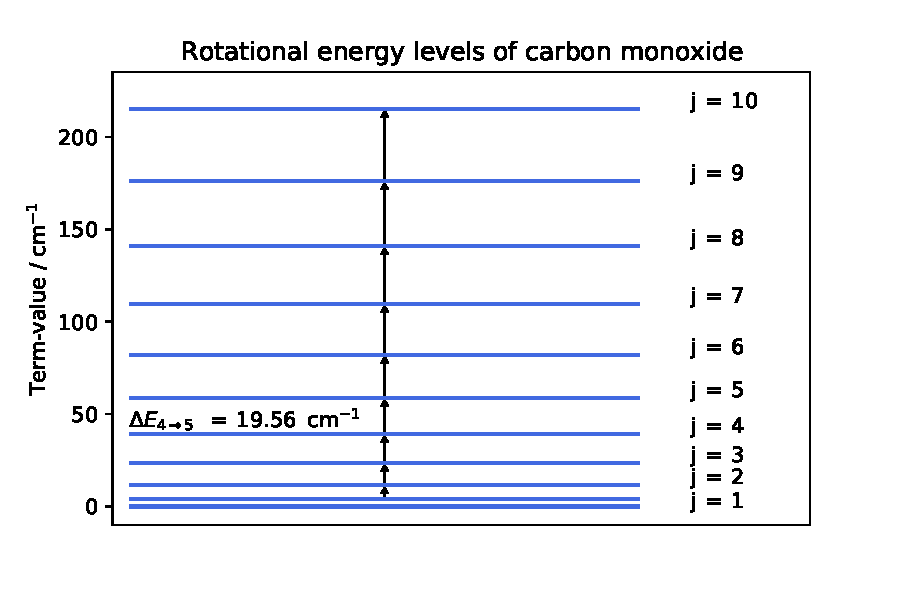
\includegraphics[width=0.9\textwidth]{/Rotation-Spectra/Rotational_energy_levels_co}
	\caption{Shown are the rotational term-values of carbon monoxide for j = $\{0,..,10\}$. The rotational constants B$_e$ and C$_e$ were calculated using the atomic masses of carbon and oxygen (12 and 16 atomic masses), an inter nuclear distance of 112 pm and an approximated spring constant of k=$2.3\cdot10^{-23}\frac{N}{m}$.}
	\label{Figure:Rotation_spectrum-Co}
\end{figure}
\subsection{Vibration spectra}
The vibrational energy levels of molecules can be determined by solving the Schr$\text{\"o}$dinger using the Born Oppenheimer approximation. The movement of the nuclei is slow compared to the electrons velocity, meaning that the electrons can adjust immediately to new nuclei distances. Resulting in minimal perturbation of the electrons by the nuclei. Based on this argument the electronic and nuclear wave-functions can be separated and solved individually.
 \begin{equation}
\Psi_{\text{total}} = \Psi_{\text{nuclei}}(R_j)\cdot \Psi_{e^-}(r_j,R_j)
\label{Born-oppenheimer}
\end{equation}
The vibration is carried out by the nuclei of the molecule and the respective Schr$\text{\"o}$dinger equation, in center of mass coordinates, becomes:
\begin{equation}
\left( \frac{\hbar^2}{2 M} \Delta^2 + E_{\text{pot}}\right) \cdot \Psi_{\text{nuclei}}(R) = E \cdot \Psi_{\text{nuclei}}(R)
\label{Schroedinger-equation-vibration_1}
\end{equation}
A separation of variables (angle and radius) can be performed to determine the behavior of the radial nuclear wave function (S(R)) and its energy eigenvalues.
\begin{equation}
\frac{1}{R^2} \frac{d}{dR} \left(R^2 \frac{dS}{dR} \right) +\frac{2 M}{\hbar}\left(E-E_{\text{pot}} -E_{\text{rot}} \right) S = 0
\label{Schroedinger-equation-vibration_2}
\end{equation}
For a pure vibration the rotational energy E$_{\text{rot}}$ (see eq. \ref{rotation_energy_levels}) is zero and the potential energy acting on the nuclei can be approximated with a Morse-potential:
\begin{equation}
E_{\text{pot}} = D_e\left(1-e^{-\alpha(R-R_e)}\right)^2
\label{Morse-potential}
\end{equation}
with the bond-dissociation energy D$_e$, the equilibrium distance of the nuclei R$_e$ and the constant $\alpha= \sqrt{\frac{k_e}{D_e}}$ described by the force-constant k$_e$.\\\\ The Schrödinger equation can be solved analytically after inputting the the Morse potential and the resulting energy eigenvalues and vibrational term-values are:
 \begin{align}
E_{vib} &= \hbar \omega (\nu +\frac{1}{2}) - \frac{\hbar^2 \omega^2}{4 D_e} (\nu +\frac{1}{2})^2 \\
F_{vib}&= \frac{E_{vib}}{h\cdot c} = \omega_e (\nu +\frac{1}{2}) - \chi_e \omega_e (\nu +\frac{1}{2})^2 
 \label{vibration_energy_eigenvalues}
 \end{align}
During the calculation the vibrational quantum number $\nu$ and the vibration frequency $\omega$ have been introduced. With the dipole selection rule: $\nu = \{0,\pm1,\pm2,...\}$ one can determine the transition energies of two adjacent vibrational energy levels:
\begin{align}
\begin{split}
\Delta F &= \frac{\Delta E}{h\cdot c} = \omega_e -2\omega_e \chi (\nu +1)
\label{vibration_transition_energy}
\end{split}
\end{align}
In contrast to the energy level splitting of the purely rotational spectra, the vibrational energy level distance $\Delta$F decreases in magnitude as the vibrational quantum number increases. Figure \ref{Figure:Morse-potential} shows the vibrational spectrum of carbon monoxide. The transition energies between two adjacent vibrational states are almost 2 orders of magnitude larger than those of two adjacent rotational energy levels (for j,$\nu$ $\leq$ 10).
\begin{figure}[H]
	\centering
	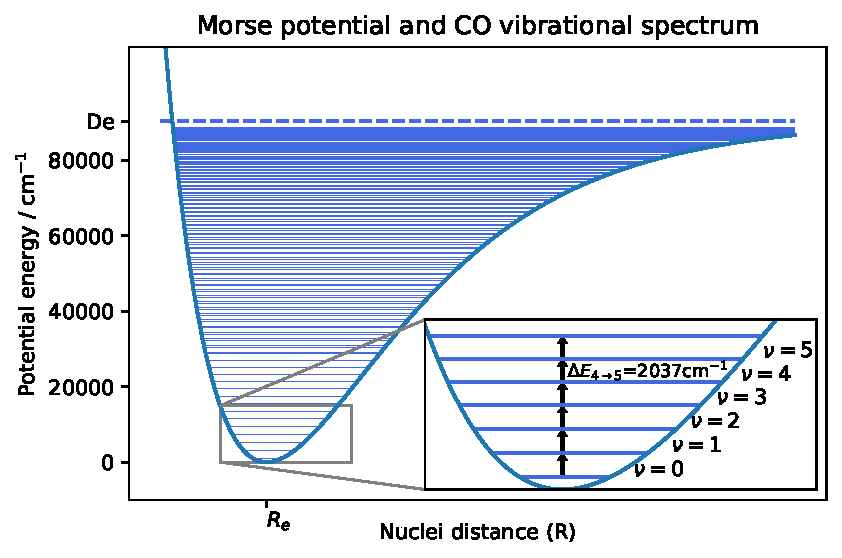
\includegraphics[width=0.9\textwidth]{/Vibration-Spectra/Morse-potential_neu}
	\caption{Shown is a Morse potential with several vibrational energy levels. The transition energy $\Delta$E decreases for increasing vibrational quantum numbers $\nu$. Vibrational energy levels beyond the dissociation energy D$_e$ do not exist. }
	\label{Figure:Morse-potential}
\end{figure}
\subsection{Rotational and vibrational spectra}
Naturally, molecules rotate and vibrate simultaneously resulting in a combined ro-vibrational absorption spectrum. The term-values can be approximated by the total energy of the motion which is given by the sum of the rotation and the vibration energy of the molecule (eq. \ref{vibration_energy_eigenvalues} and eq. \ref{rotation_energy_levels_cm-1_final}):
\begin{align}
\begin{split}
	E &= E_{rot} + E_{vib} \\
	F &= \omega_e (\nu +\frac{1}{2}) - \chi_e \omega_e (\nu +\frac{1}{2})^2 + B_e \cdot j(j+1) -  C_e \cdot j^2(j+1)^2 
\label{term-values-rovibration-spectrum}
\end{split}
\end{align}
The ro-vibrational term-values are completely defined by the four molecular constants ($\omega_e$, $\chi_e$, B$_e$ and C$_e$) and the two quantum numbers $\nu$ and j. The individual energy levels of the spectrum are separated into 3 branches, based on transition rules ($\Delta j =0, \pm1 $ and $\Delta \nu =\pm1 $) and transition energies.\\ \\
The \textbf{Q-branch} includes ro-vibrational transitions for which only the vibrational quantum number changes ($\Delta \nu = \pm 1$), while the rotational quantum number remains the same ($\Delta$ j= 0). The photon energy, that is required to induce a Q-branch transition, is therefore identical to the respective vibrational term-values $\Delta$F$_{vib}$. (see eq. \ref{vibration_transition_energy}). Thus the Q-branch only consists of a single absorption line which is energetically located in between the P- and the R-branch transitions.\\ \\
The \textbf{P-branch} transitions requires less energy than the Q-branch transition, since the rotational quantum number j changes by -1, resulting in an overall energy decrease. 
\\ \\The \textbf{R-branch} contains all ro-vibrational transitions, where the rotational quantum number is increased by +1 during the transition. The required energy is larger than the respective purely vibrational transition energy. \\\\ 
Figure \ref{Figure:ro-vi-spectrum} shows the rotational and vibrational term-values of carbon monoxide with an expemplaric Q-, R- and P-branch transition.
\begin{figure}[H]
	\centering
	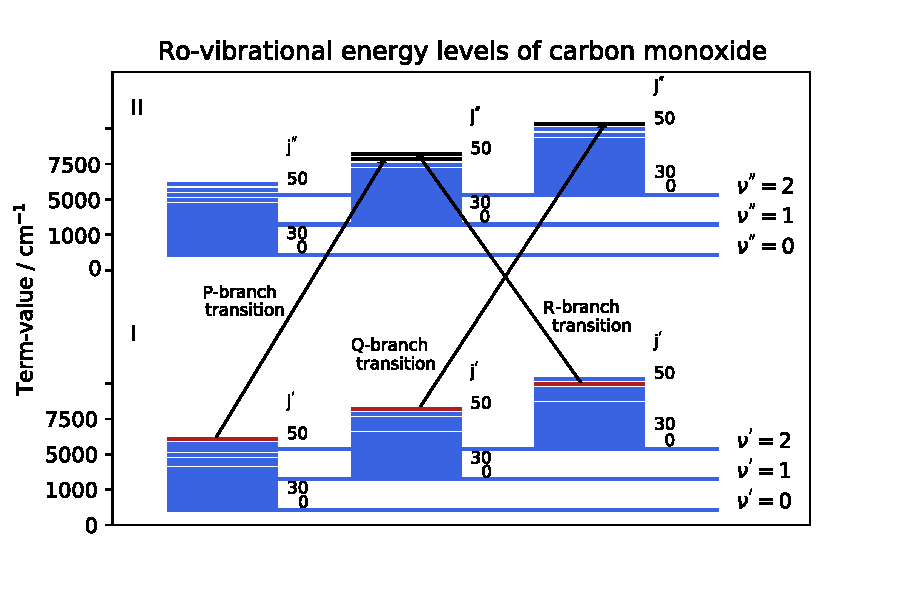
\includegraphics[width=0.9\textwidth]{/Ro-vi-Spectra/Ro-vi_energy_levels_co_ver3}
	\caption{Shown are the ro-vibrational states I and II with their respective quantum numbers: j$^{\prime}$, $\nu^{\prime}$, and j$^{\prime \prime}$, $\nu^{\prime \prime}$. Three possible transitions are indicated with arrows and each can be related to one of the three branches respectively. The shown P-branch transition (with $\Delta j_{(50 \rightarrow 49)}=-1$ and $\Delta \nu_{(0 \rightarrow 1)}=+1$)  requires less energy than the Q-branch transition (with $\Delta j_{(50 \rightarrow 50)}=0$ and $\Delta \nu_{(1 \rightarrow 2)}=+1$) which is energetically equal to the pure vibrational transition with $\Delta \nu_{(1 \rightarrow 2)}=+1$. The R-branch transition (with $\Delta j_{(49 \rightarrow 50)}=+1$ and $\Delta \nu_{(2 \rightarrow 1)}=-1$) requires the highest energy. }
	\label{Figure:ro-vi-spectrum}
\end{figure}
\subsection{HITRAN database}
The high-resolution transmission molecular absorption database, short HITRAN, is a database that contains spectroscopic parameters of roughly 50 molecules and their respective isotopes. Some important parameters that are included for most absorption lines are: the central wavelength ($\nu_{ij}$), the line strength (S), the self and air broadened linewidth ($\gamma_{self}$ and  $\gamma_{air}$) and the pressure shift $\delta_{air}$. The database is updated continuously with the most recent and most accurate experimental results which were generated by various experimental setups e.g Fourier transform infrared spectroscopy but also other like cavity ring-down spectroscopy or tunable diode Laser absorption spectroscopy. The database is maintained by the Harvard and Smithsonian center for astrophysics and a publishable summary of the recent changes is disclosed every four years. With the most recent publication being submitted in 2016 \cite{Hitran2016}. Figure \ref{CO2_Absorbtion_HITRAN} shows an exemplaric absorption spectrum of CO and its isotopes in the mid infrared region, which was taken from the HITRAN database.
\begin{figure}[H]
	\centering
	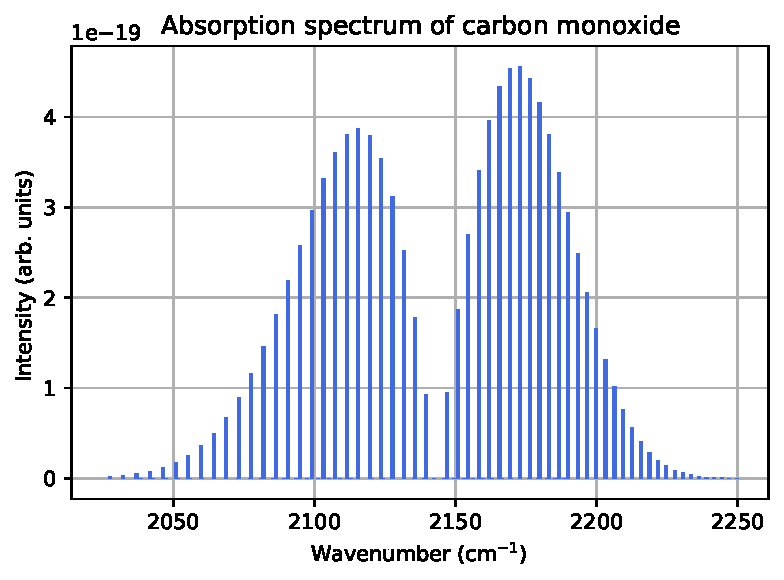
\includegraphics[width=0.9\textwidth]{/HITRAN-Linewidth-and-absorption/Absorption_of_CO_and_CO_isotopes}
	\caption{Shown are the P- and R-branch of CO in the mid infrared region. The data was taken from the HITRAN database \cite{Hitran2012} \cite{Hitran2016}.}
	\label{CO2_Absorbtion_HITRAN}
\end{figure}
\section{Spectral line shapes}
Line shapes and especially line widths of radiating transitions are described by the full-width-half-maximum (FWHM) of the respective line shape function. The corresponding line shape function on the other hand can greatly depend on environmental influences such as temperature and pressure but it is also influenced by natural radiation characteristics of atoms.
\subsection{Natural line broadening}
The natural line width is the minimal finite linewidth that any spectral line has, independent of environmental influences. An excited atom or molecule that emits lights can be described in classical terms by a damped dipole oscillation and this damped radiation process is responsible for the existence of the natural line width. \\ \\In the classical model the oscillator has the mass $m$ and the Eigenfrequency $\omega_0=\sqrt{d/m}$, which is related to the spring constant d. Solving the differential equation of the damped harmonic oscillator:
\begin{equation}
\ddot{x}+\gamma \dot{x}+ \omega_0^2x=0
\label{Bewegungsgleichung_gedaemfte_schwingung}
\end{equation}
yields the solution for the time dependent behavior of the oscillation x(t):
\begin{equation}
x(t)=x_0 e^{-\frac{\gamma t}{2}}(\cos(\omega t)+\frac{\gamma \omega}{2}\sin(\omega t))
\label{Bewegungsgleichung_gedaemfte_schwingung_loesung}
\end{equation}
with the damping coefficient $\gamma$ and the frequency $\omega=\sqrt{\omega_0^2-(\frac{\gamma}{2})^2}$. In general $\gamma\ll\omega_0$ holds true and  \ref{Bewegungsgleichung_gedaemfte_schwingung_loesung} can be further simplified to:
\begin{equation}
x(t)\approx x_0 e^{-\frac{\gamma t}{2}} \cos(\omega_0 t)
\label{Bewegungsgleichung_gedaemfte_schwingung_loesung_naeherung}
\end{equation}
The exponentially decreasing amplitude of the oscillation is responsible for a spectral broadening of the emitted light around the central frequency $\omega_0$ and the Fourier-transformation of \ref{Bewegungsgleichung_gedaemfte_schwingung_loesung_naeherung} will give rise about the exact spectral line shape of the observed electro-magnetic transition. The spectral amplitude $A(\omega)$ is given by:
\begin{align}
A(\omega) &=\frac{1}{\sqrt{2\pi}}\int_{0}^{\infty}x_0 e^{-\frac{\gamma t}{2}} \cos(\omega_0 t) e^{-i\omega t} dt \nonumber \\
A(\omega) &=\frac{x_0}{\sqrt{8\pi}}\left(\frac{1}{i(\omega_0-\omega)+\frac{\gamma}{2}}+\frac{1}{i(\omega_0+\omega)+\frac{\gamma}{2}}\right) \nonumber\\
A(\omega) &\approx\frac{x_0}{\sqrt{8\pi}}\left(\frac{1}{i(\omega_0-\omega)+\frac{\gamma}{2}}\right) \text{, for }  (\omega-\omega_0) \ll \omega_0 \\
\label{Fouriertransformation_a(omega)}\nonumber
\end{align}
and it can be used to calculate the spectral intensity I($\omega$), which is proportional to $|A(\omega)|^2$.
\begin{equation}
I(\omega) \propto |A(\omega)|^2 = \frac{\gamma/2\pi}{(\omega-\omega_0)^2+(\frac{\gamma}{2})^2}
\label{Intensitaet_}
\end{equation}
The natural line shape function $I(\omega)$ has a characteristic Lorentz shape and its FWHM is defined as the natural linewidth of the respective EM-transition. Due to the finite radiation time of the atoms, any absorption or emission line has a natural line width which is furthermore independent of any environmental influences. \\ \\ The existence of the natural line width can also be explained using Heisenberg's uncertainty principle, where the energy uncertainty is rewritten as frequency uncertainty: 
\begin{equation}
 \Delta \nu \geq \frac{1}{2 \pi \Delta t}
\label{Heisenberg_unscharfe}
\end{equation}
The principle in this form states, that the frequency uncertainty of a radiating transition between an excited state, with the energy $E_i$ and the life time $\tau_i= \Delta t$,  and the ground state will be greater than zero. Which is due to the fact that all excited states have finite life times. Radiating transitions between two excited states have greater natural line widths since their individual energy uncertainties are additive.



\subsection{Temperature dependent line broadening}
The natural line broadening is present for every radiative transition and is usually superimposed with additional line broadening effects. One additional effect is the temperature broadening (also called Doppler broadening) effect of a transition line. It is present for in many absorption and emission lines of gasses and usually dominates the pressure broadening effect at low pressure values. \\ \\
Considering an ideal gas with radiating atoms, the gas-particles are generally moving with a velocity $\vec{v} > 0$ while they emit light with the central frequency $\omega_0$. For a static observer (i.e another atom) this movement results in a frequency shift of the incoming light due to the Doppler-effect:
\begin{equation}
\omega_{obs}= \omega_0 +\vec{k} \cdot \vec{v}
\label{Doppler_effect}
\end{equation}
The same holds true for atoms which move with a velocity $\vec{v}$ and absorb light during the movement. Their absorbtion frequency is shifted according to the Doppler-effect and only light with the frequency $\omega=\omega_{obs}$ can induce the atomic transition. \\ \\ If the system is in thermal equilibrium the gas-particle velocities can be described by the Maxwell-distribution. The density of absorbing gas-molecules which are in the atomic state $E_i$ is then given accordingly by:
\begin{equation}
n_i(v_z)dv_z = \frac{N_i}{\sqrt{2k_bT/m}} \ e^{-(\frac{v_z}{\sqrt{2k_bT/m}})^2}dv_z
\label{Maxwell_geschwindigkeitsverteilung}
\end{equation}
The spectral intensity $I(\omega)$ is proportional to $n(\omega)$, which can be calculated by inserting \ref{Doppler_effect} into \ref{Maxwell_geschwindigkeitsverteilung}. The calculation yields:
\begin{equation}
I(\omega)=I(\omega_0) \ e^{-\left(\frac{c(\omega-\omega_0)}{\omega_0\sqrt{2k_bT/m}}\right)^2}
\label{Doppler_verbreiterung}
\end{equation}
The resulting line shape is a Gaussian function with the corresponding Doppler broadened line width $\Delta \omega = \frac{\omega_0}{c}\sqrt{(8k_bTln2)/m}$. In contrary to the natural line width, the Doppler line width depents on multiple environmental factors including the temperature, particle mass and the central frequency $\omega_0$. 



\subsection{Pressure dependent line broadening and line shift}
\noindent
If the atoms  of a radiating gas are introduced to foreign gas molecules, their individual energy levels are shifted whenever the two species interact with each other. This energy shift greatly depends on the electrical properties of the two interacting particles and their distance $R$ to each other. If one considers a radiating transition between the energy levels $E_i$ and $E_k$ of the host atoms, one can observe positive and negative energy shifts relative to the initial energy of the two states. This is due to the different types of electrostatic interactions between the native and the perturbating molecules. Van der Waals forces, generated by the interaction with the perturbating molecules, will result in a negative energy shift of $E_i$ and $E_k$. While positve energy shifts are introduced by electrostatic repulsion. The distortion of the energy levels is usually greater for higher levels which results in a net change of the central transition frequency $\nu_0$ \cite{Margenau1936}. 
The schematic potential curves of $E_i$ and $E_k$ are presented in Figure \ref{figure:lennard_jones_bild_druck_verbreiterung} for different values of $R$ and the altered transition frequencies that are generated due to the quasi collision of the particles. If the system is in thermal equilibrium the relative core distances are distributed around a mean value $R_m$, which eventually results in the broadening of the transition line around a central transition frequency $\nu_m$. \\
\begin{figure}[ht]
	\centering
	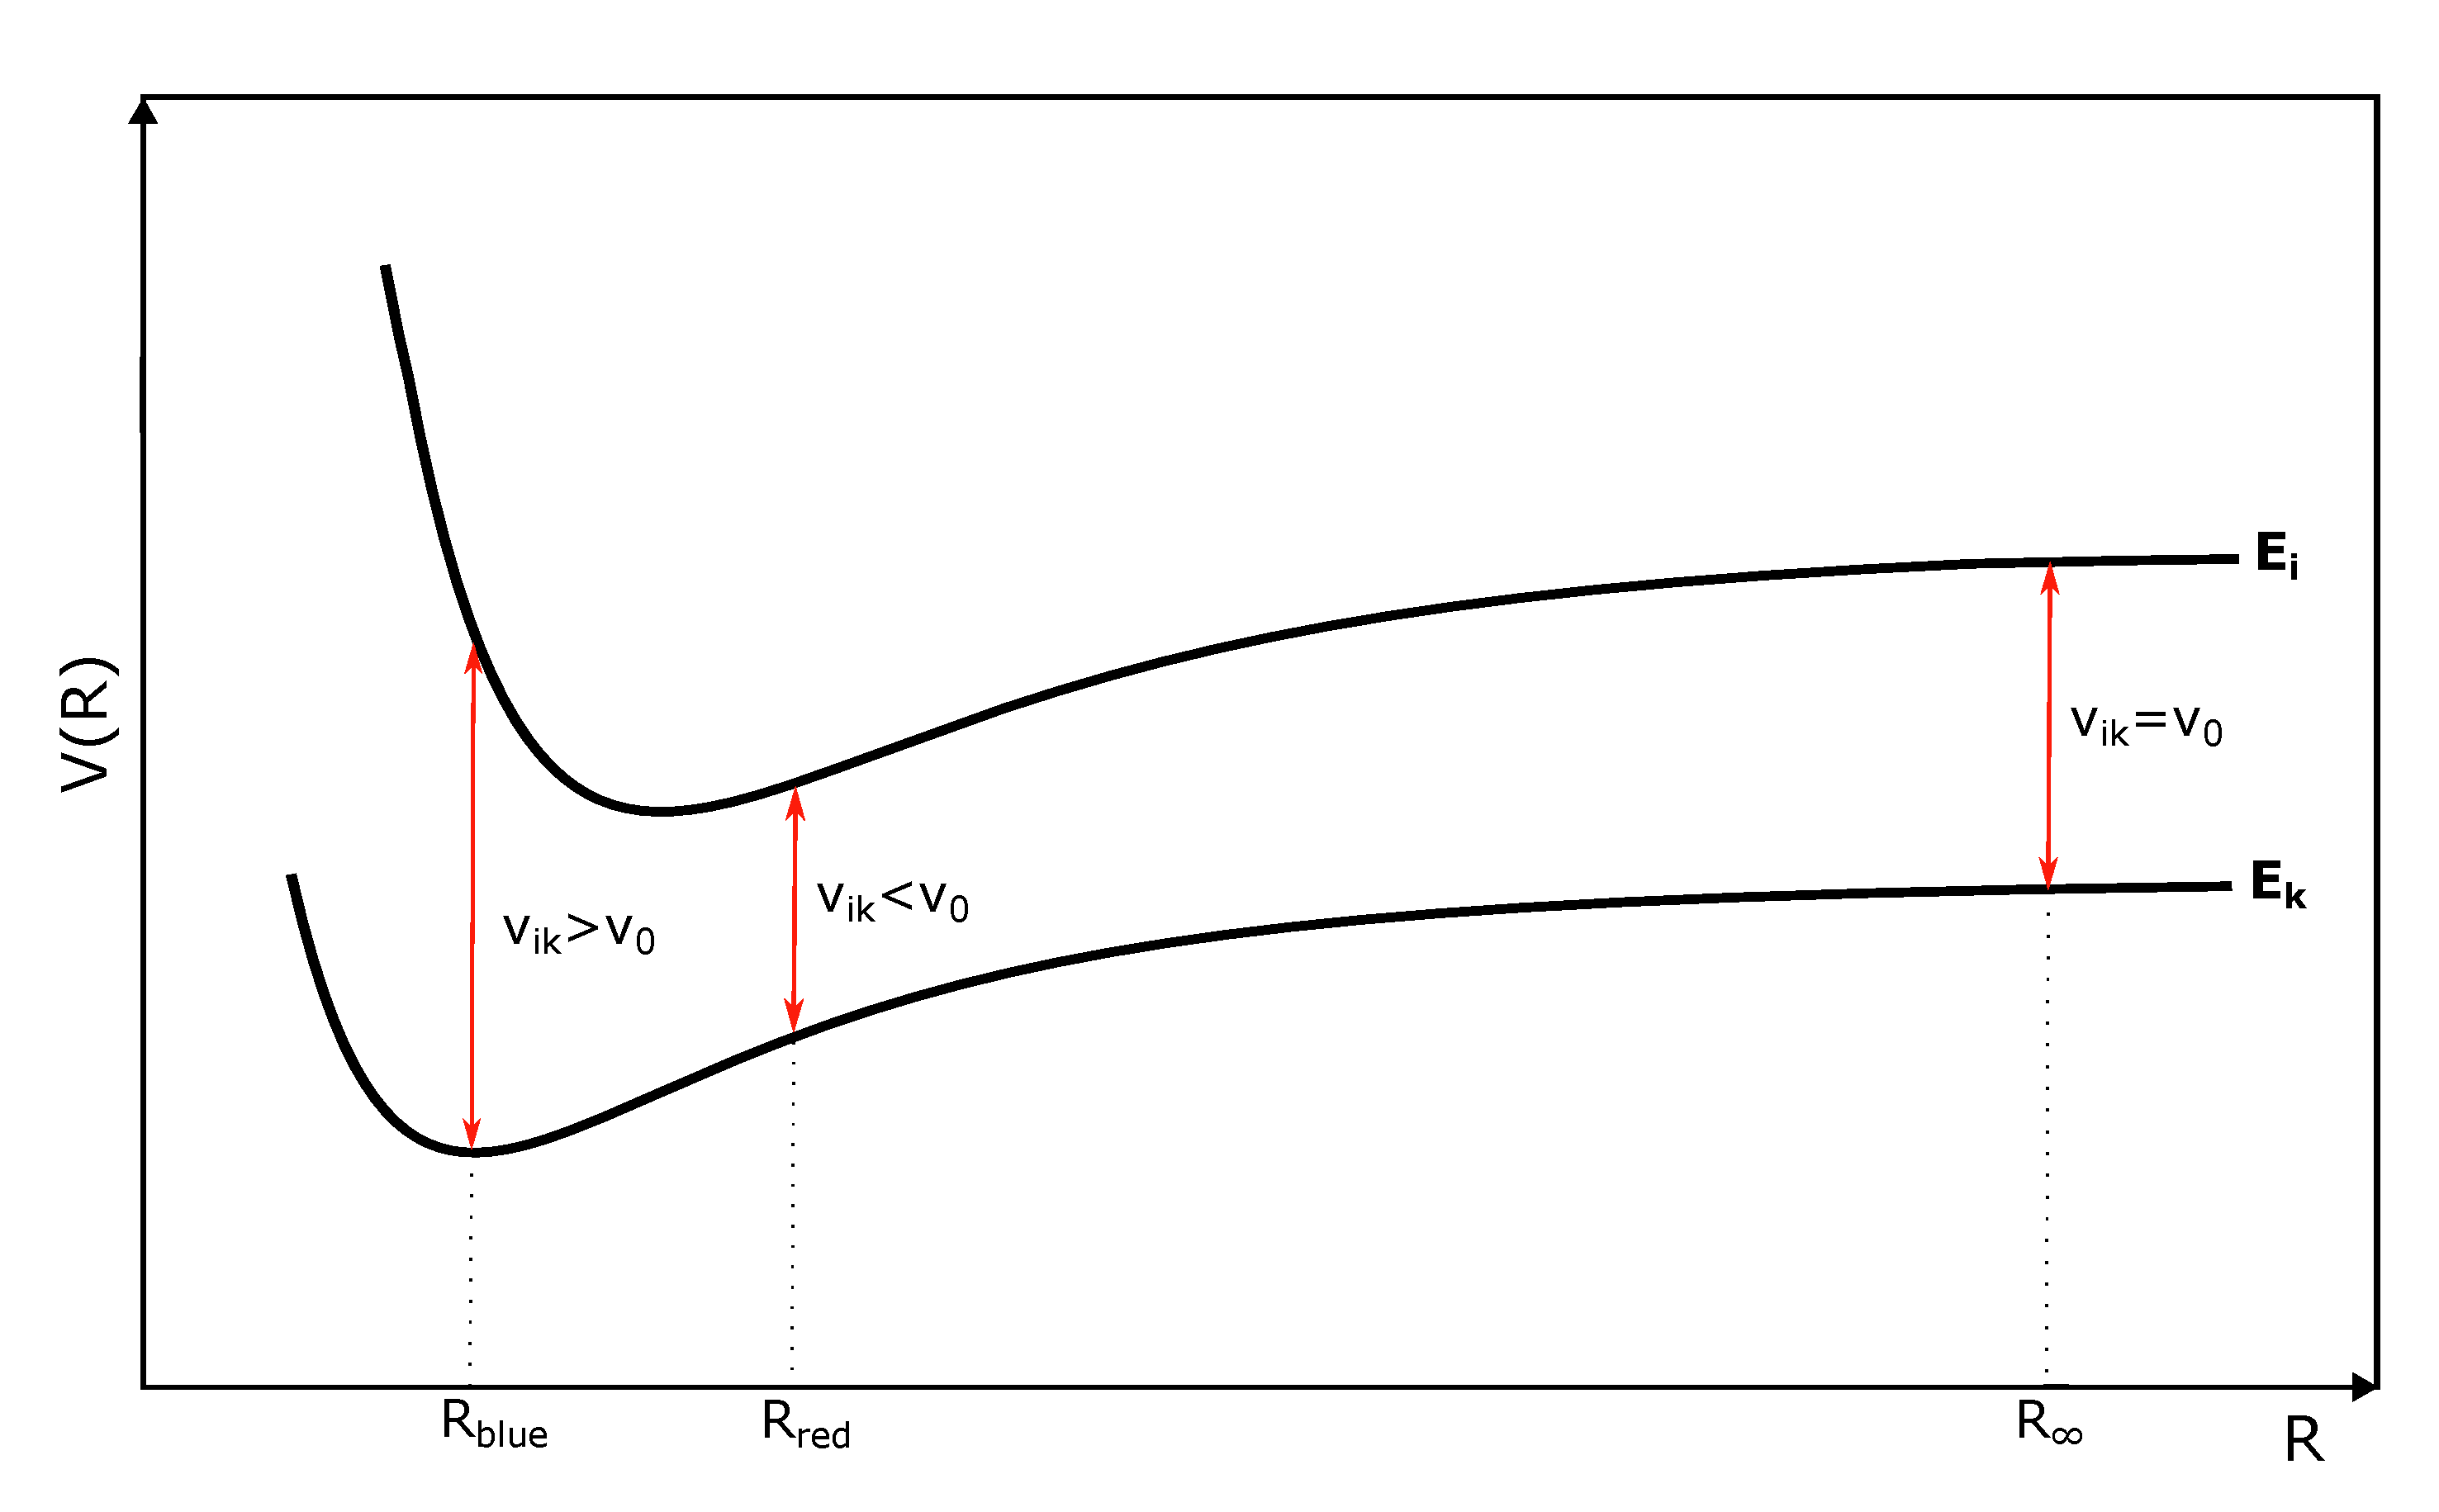
\includegraphics[width=0.75\textwidth]{Optic-Theorie/Lennard_jones_bild_druck_verbreiterung}
	\caption{Shown are the (Lenard-Jones) potential-curves of the two energy levels $E_i$ and $E_k$ while they are subject to the perturbation of a foreign atom. If the atoms are reasonably separated (for $R=R_\infty$) the transition frequency $\nu_{ik}$ remains unchanged and is equal to $\nu_0$. In most cases the transition frequency is shifted to the red (for $R=R_{red}$) while in rare occasions blue shifts are also present (for $R=R_{blue}$).}
	\label{figure:lennard_jones_bild_druck_verbreiterung}
\end{figure}\\ 
In 1932 F. Weisskopf described the collision dependent line broadening and line shift in classical terms \cite{Weisskopf1932}. He considered a damped harmonic oscillator with an additional collision dependent damping constant. The collision of the two particles contributes to a phase change $\Theta$ of the oscillating native gas particle. The phase change introduces a change of oscillation frequency while the atoms collide. This makes the frequency a time dependent variable. The waveform $x(t)$ that describes the time dependent behavior of the collision damped oscillator is then given by:
\begin{equation}
x(t)=x_0\cdot e^{-i\int_{0}^{t}\omega(t')dt'}
\label{Bewegungsgleichung_collision_damped_oscillator}
\end{equation}
A Fourier-transformation of eq: \ref{Bewegungsgleichung_collision_damped_oscillator} yields the spectral amplitude $A(\omega)$ and the squared absolute value of $A(\omega)$ is proportional to the desired spectral line shape $I(\omega)$: 
\begin{equation}
I(\omega) d\omega =\frac{2}{3}\frac{e^2\omega^4}{c^3} \frac{1}{2\pi}\ \left|\int_{-\infty}^{\infty} x_0\cdot e^{-i\int_{0}^{t}\omega(t')dt'} \cdot e^{i\omega t} dt \right|^2d\omega
\label{Spectral_amplitude_collision_damped_oscillator}
\end{equation}
The prefactor in eq: \ref{Spectral_amplitude_collision_damped_oscillator} is determined classicaly from the radiation characteristics of an oscillating charge. Solving the integral yields the final Lorentzian-shaped result for the collision broadened line intensity  $I(\omega)$ :
\begin{equation}
	I(\omega)=\frac{2\omega^4e^2x_0^2}{3\pi c^3}\cdot \frac{(1-A)/\tau_c}{\left((1-A)/\tau_c\right)^2+\left(B/\tau_c-( \omega-\omega_0) \right)^2}
	\label{Linienform_collision_damped_oscillator}
\end{equation}
with the factors A and B that describe the phase shifts which occur due to the collisions: $A=\int_{-\infty}^{\infty} \rho(\Theta) \cos(\Theta) d\Theta $ and $B=\int_{-\infty}^{\infty} \rho(\Theta) \sin(\Theta) d\Theta $. The coefficient $\rho(\theta)\ d\Theta$ is the probability that a phase shift occurs within the phase interval $\Delta\Theta= \Theta+d \Theta$ and $\tau_c$ is the mean free time between collisions.
The full calculation with an additional overview of the quantum mechanical approach for the problem is described in detail in \cite{chen1957}.\\ \\ 
The frequency shift $\Delta \nu$ and the half-width $\delta \nu$ are related to the                                           coefficients A and B are given by: 
\begin{align}
\Delta \nu&=\int_{0}^{\infty} \rho(\Theta)\cdot \left( 1-\cos(\Theta)\right)/\tau_c \ d\Theta  \\
\delta \nu&=\int_{0}^{\infty} \rho(\Theta)\cdot \sin(\Theta)/\tau_c \ d\Theta \\ \nonumber
\end{align}
Both, the line width and the line shift are proportional to the particle density. The function $\frac{\rho(\Theta) \ d\Theta }{ \tau_c}$ can be understood as the number of collisions during the mean free time $\tau_c$, which greatly depends on the gas density. The gas density on the other hand is related to the gas pressure and temperature via the ideal gas law, which is the reason why the collision broadening is often called pressure broadening. 
\subsection{Combined effects}
Under realistic measurement conditions (e.g at room temperature and atmospheric pressure), the actual spectral line shape will be influenced by the temperature and pressure simultaneously. The line shape function can then be described by a Voigt-profile to accommodate for both effects. A Voigt profile results from the convolution of a Gaussian and a Lorentzian function:
\begin{equation}
\text{V($\omega$, P, T)}=\text{G($\omega$, T)} *\text{L($\omega$, P)}  = \int_{-\infty}^{\infty} \text{G($\tau$, T)}  \cdot \text{L($\omega-$$\tau$, P)} d\tau
\label{Voigt-profile}
\end{equation}
Figure \ref{figure:comparison_line_shapes} shows a comparison of three previously describes spectral line shape functions.\\\\ Although a Voigt profile is a good first approximation of the physical situation, it has become apparent over the last decades that it does not adequately describe the experimentally generated results.  For a more detailed description one has to also consider the mutual interference of the Doppler and collision broadening, which both depend on the particle velocity. This can, for example, lead to a particle being 
\begin{figure}[ht]
	\centering
	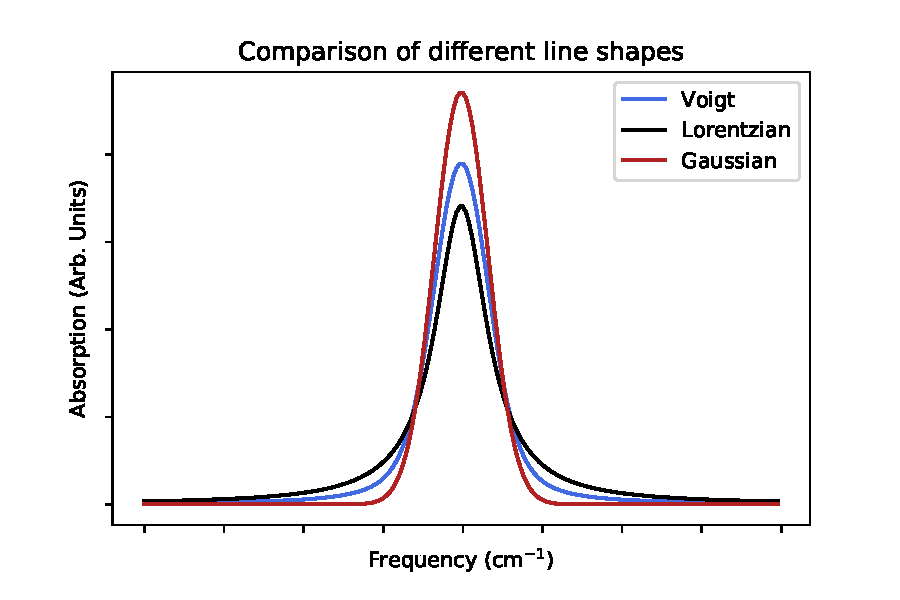
\includegraphics[width=0.9\textwidth]{Optic-Theorie/Comparison_of_different_lane_shapes}
	\caption{Shown are the Voigt-, Lorentzian- and Gaussian-spectral-line-shapes with area normalized profiles.}
	\label{figure:comparison_line_shapes}
\end{figure}
\section{Multipass absorption cells}
Multi pass absorption cells are used to increase the optical pathways within an absorption spectroscopy setup. While the light travels through the active medium more and more light intensity is lost due to absorption processes. To be able to detect low gas densities (eg of atmospheric greenhouse gases) one requires great optical path lengths since the two physical properties are inversely proportional to each other.
\begin{equation}
\rho=-Ln(\frac{I}{I_0})/(\alpha \cdot L)
\end{equation}
There are many different types of multipass absorption cells and their basic principle, as well as their main advantages and disadvantages are being discussed in the upcoming chapters.
\subsection{White cell}
The White cell was designed in 1942 by John U. White and consists of three spherical, concave mirrors \cite{White1942}. Two adjacent mirrors ($A_1$ and $A_2$) are positioned opposite to a larger mirror B. The distance between the mirrors is equal to their radius of curvature. The light is reflected $(n\cdot4)$ times within the White-cell. The integer number n can be increased or decreased by tilting the mirrors $A_1$ and $A_2$. Thereby the position of the center of curvature, on the surface of mirror B, can be adjusted to allow fewer or additional reflections. The basic operating principle of the multi reflection cell is shown in \ref{Figure:White-cell} together with the individual center curvature which are indicated in a red circles. A white-cell is capable of achieving several meters of optical path length with a simple design that requires no significant alignment of the mirrors.
\begin{figure}[H]
	\centering
	\begin{subfigure}{.5\textwidth}
		\centering
		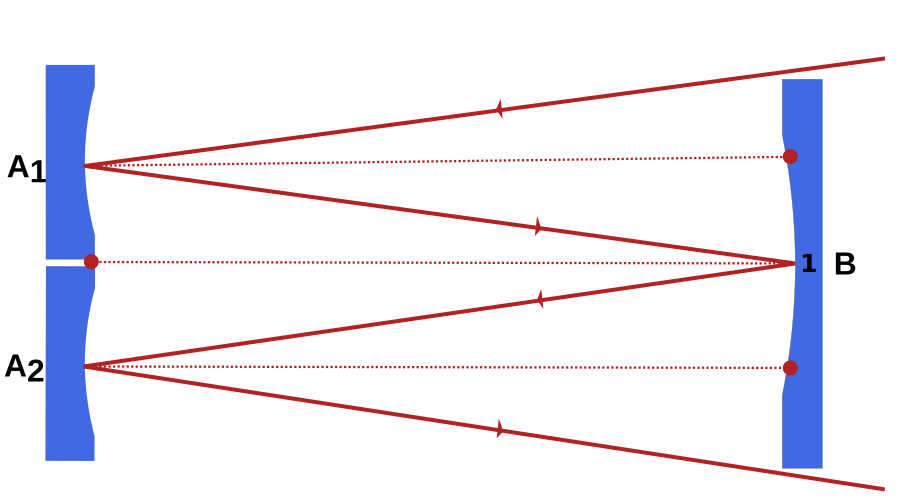
\includegraphics[width=\textwidth]{/White-cell/White-Cell-1-on-b}
		\caption{Configuration I}
	\end{subfigure}%
	\begin{subfigure}{.5\textwidth}
		\centering
		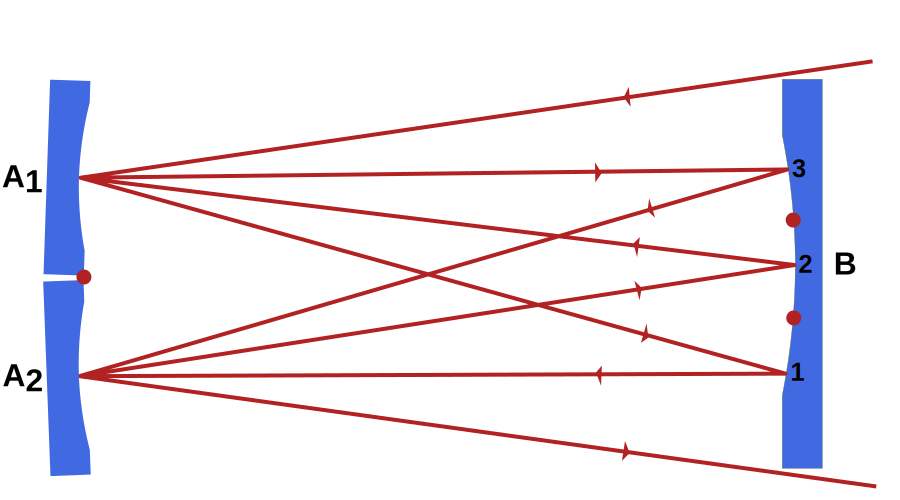
\includegraphics[width=\textwidth]{/White-cell/White-Cell-3-on-b}
		\caption{Configuration II}
	\end{subfigure}
	\caption{Shown is the basic operating principle of a White-cell, together with two possible configurations. \textbf{Configuration I}: The mirrors are close to parallel to each other and a total of four reflections are achieved. \textbf{Configuration II}: The mirrors $A_1$ and $A_2$ are slightly tilted to the center of mirror B. A total of twelve reflections are achieved in this arrangement. The reflection sequence is specified by arrows and an additional enumeration (1-3) on Mirror B.}
	\label{Figure:White-cell}
\end{figure}
\newpage
\subsection{Herriott-cell}
Herriott-cells are another commonly used type of optical multipass cells. They were invented in 1965 by Donald R. Herriott and consist of two spherical mirrors with identical focal lengths. One of the mirror has a small hole, usually between 2 and 5 mm in diameter, which is utilized to couple Laser light into the cell. The light enters the cell, is reflected from both mirror surfaces and exits the multipass cell through the same hole under a different angle, which allows for a simple spatial separation of the in and out coupled laser rays. The number of reflections on each mirror and the overall optical path length, depend on the focal lengths of the mirrors and their distance D to each other. Path lengths between a couple centimeters and several hundred meters are possible, depending on the design of the Herriott-cell. Figure \ref{Figure:Heriott-cell} shows the basic operating principle of a Herriott-Cell.
\begin{figure}[H]
	\centering
		\centering
		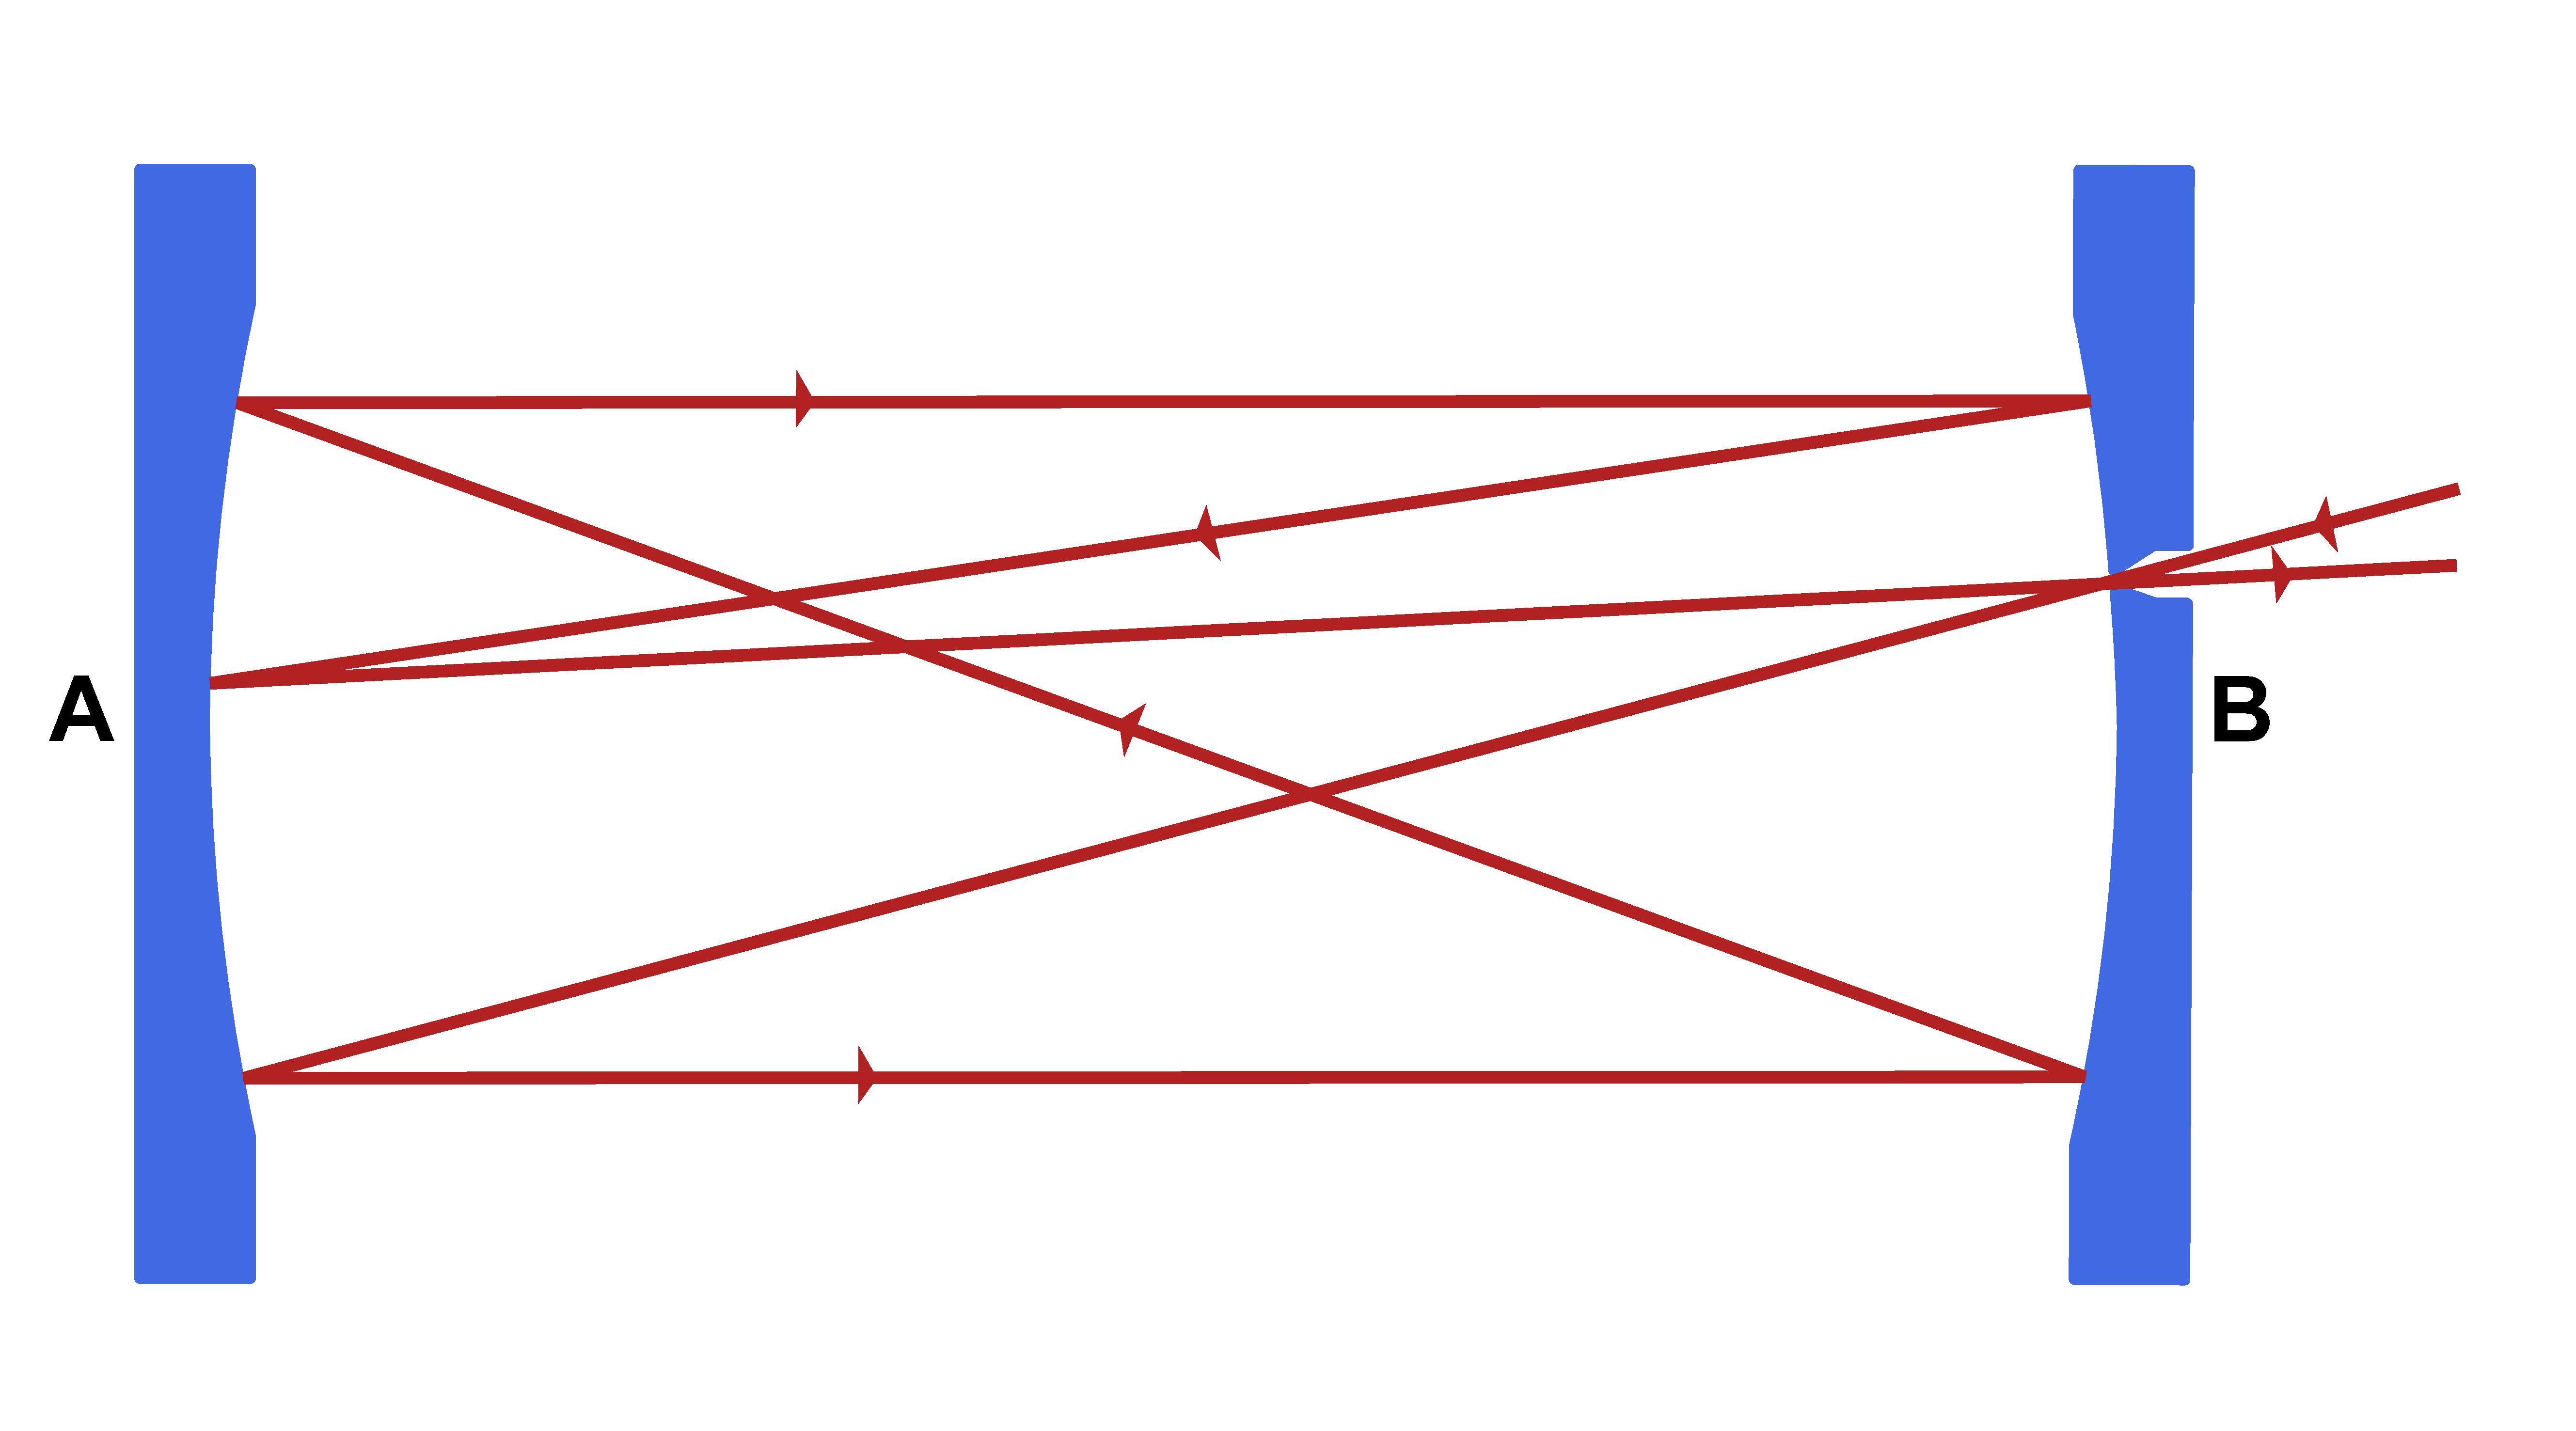
\includegraphics[width=0.7\textwidth]{/Herriott-cell/Herriott-2d}
		\caption{Shown is the basic design of a Herriott-Cell. The mirrors A and B have identical optical properties and the number of reflections on each mirror depends on the distance between the mirror and their radius of curvature.}
	\label{Figure:Heriott-cell}
\end{figure}
\noindent
Depending on the Laser's angle of incident and the distance between the mirrors, the spot pattern on the Herriott-cell mirrors are either elliptical or spherical. This allows for an exact geometrical calculation of the total optical path length, which is an important property for absorption processes. Fig\ref{Figure:Heriott-cell-geometry} introduces the necessary geometry to determine the total optical path length for a spherical spot pattern. \\\\
The "Top-View" shows the two spherical mirrors M1 and M2 in the x-z plane, which are positioned on the z-axis at a given distance D. The center of the coordinate system $(x,y,z) = (0,0,0)$ is identical to the center of the spherical mirror containing the small hole used for in-coupling the laser into the cell. The hole is located at $x_0=r_S$. The bold, purple and orange arrows show the Laser entering and leaving the Herriott-Cell and for a spherical spot pattern the beams are overlapping in the x-z plane. \\\\
The Front view on the right in Fig \ref{Figure:Heriott-cell-geometry} shows the x-y plane and illustrates the directional change of the reflected Laser beams inside of the cell. The number of reflections are labeled from 0 to 2N and change in color between red and green depending on the mirror from which the last ray was reflected. For consecutive reflections (e.g from N=1 to N=2) the Laser beam ends on the same x-positon at which the following reflection starts. The end-coordinates for the first reflection are therefore labeled as $x=r_{x1}$ and $y=r_{y1}$ with $rs^2=r_{x1}^2+r_{y1}^2$. The overall initial and final reflections are again shown by the bold, purple and orange arrows. The last reflected laser beam (orange) leaves the Herriott-Cell at the same x-position at which the first one (purple) entered. 
\begin{figure}[H]
	\centering
	\centering
	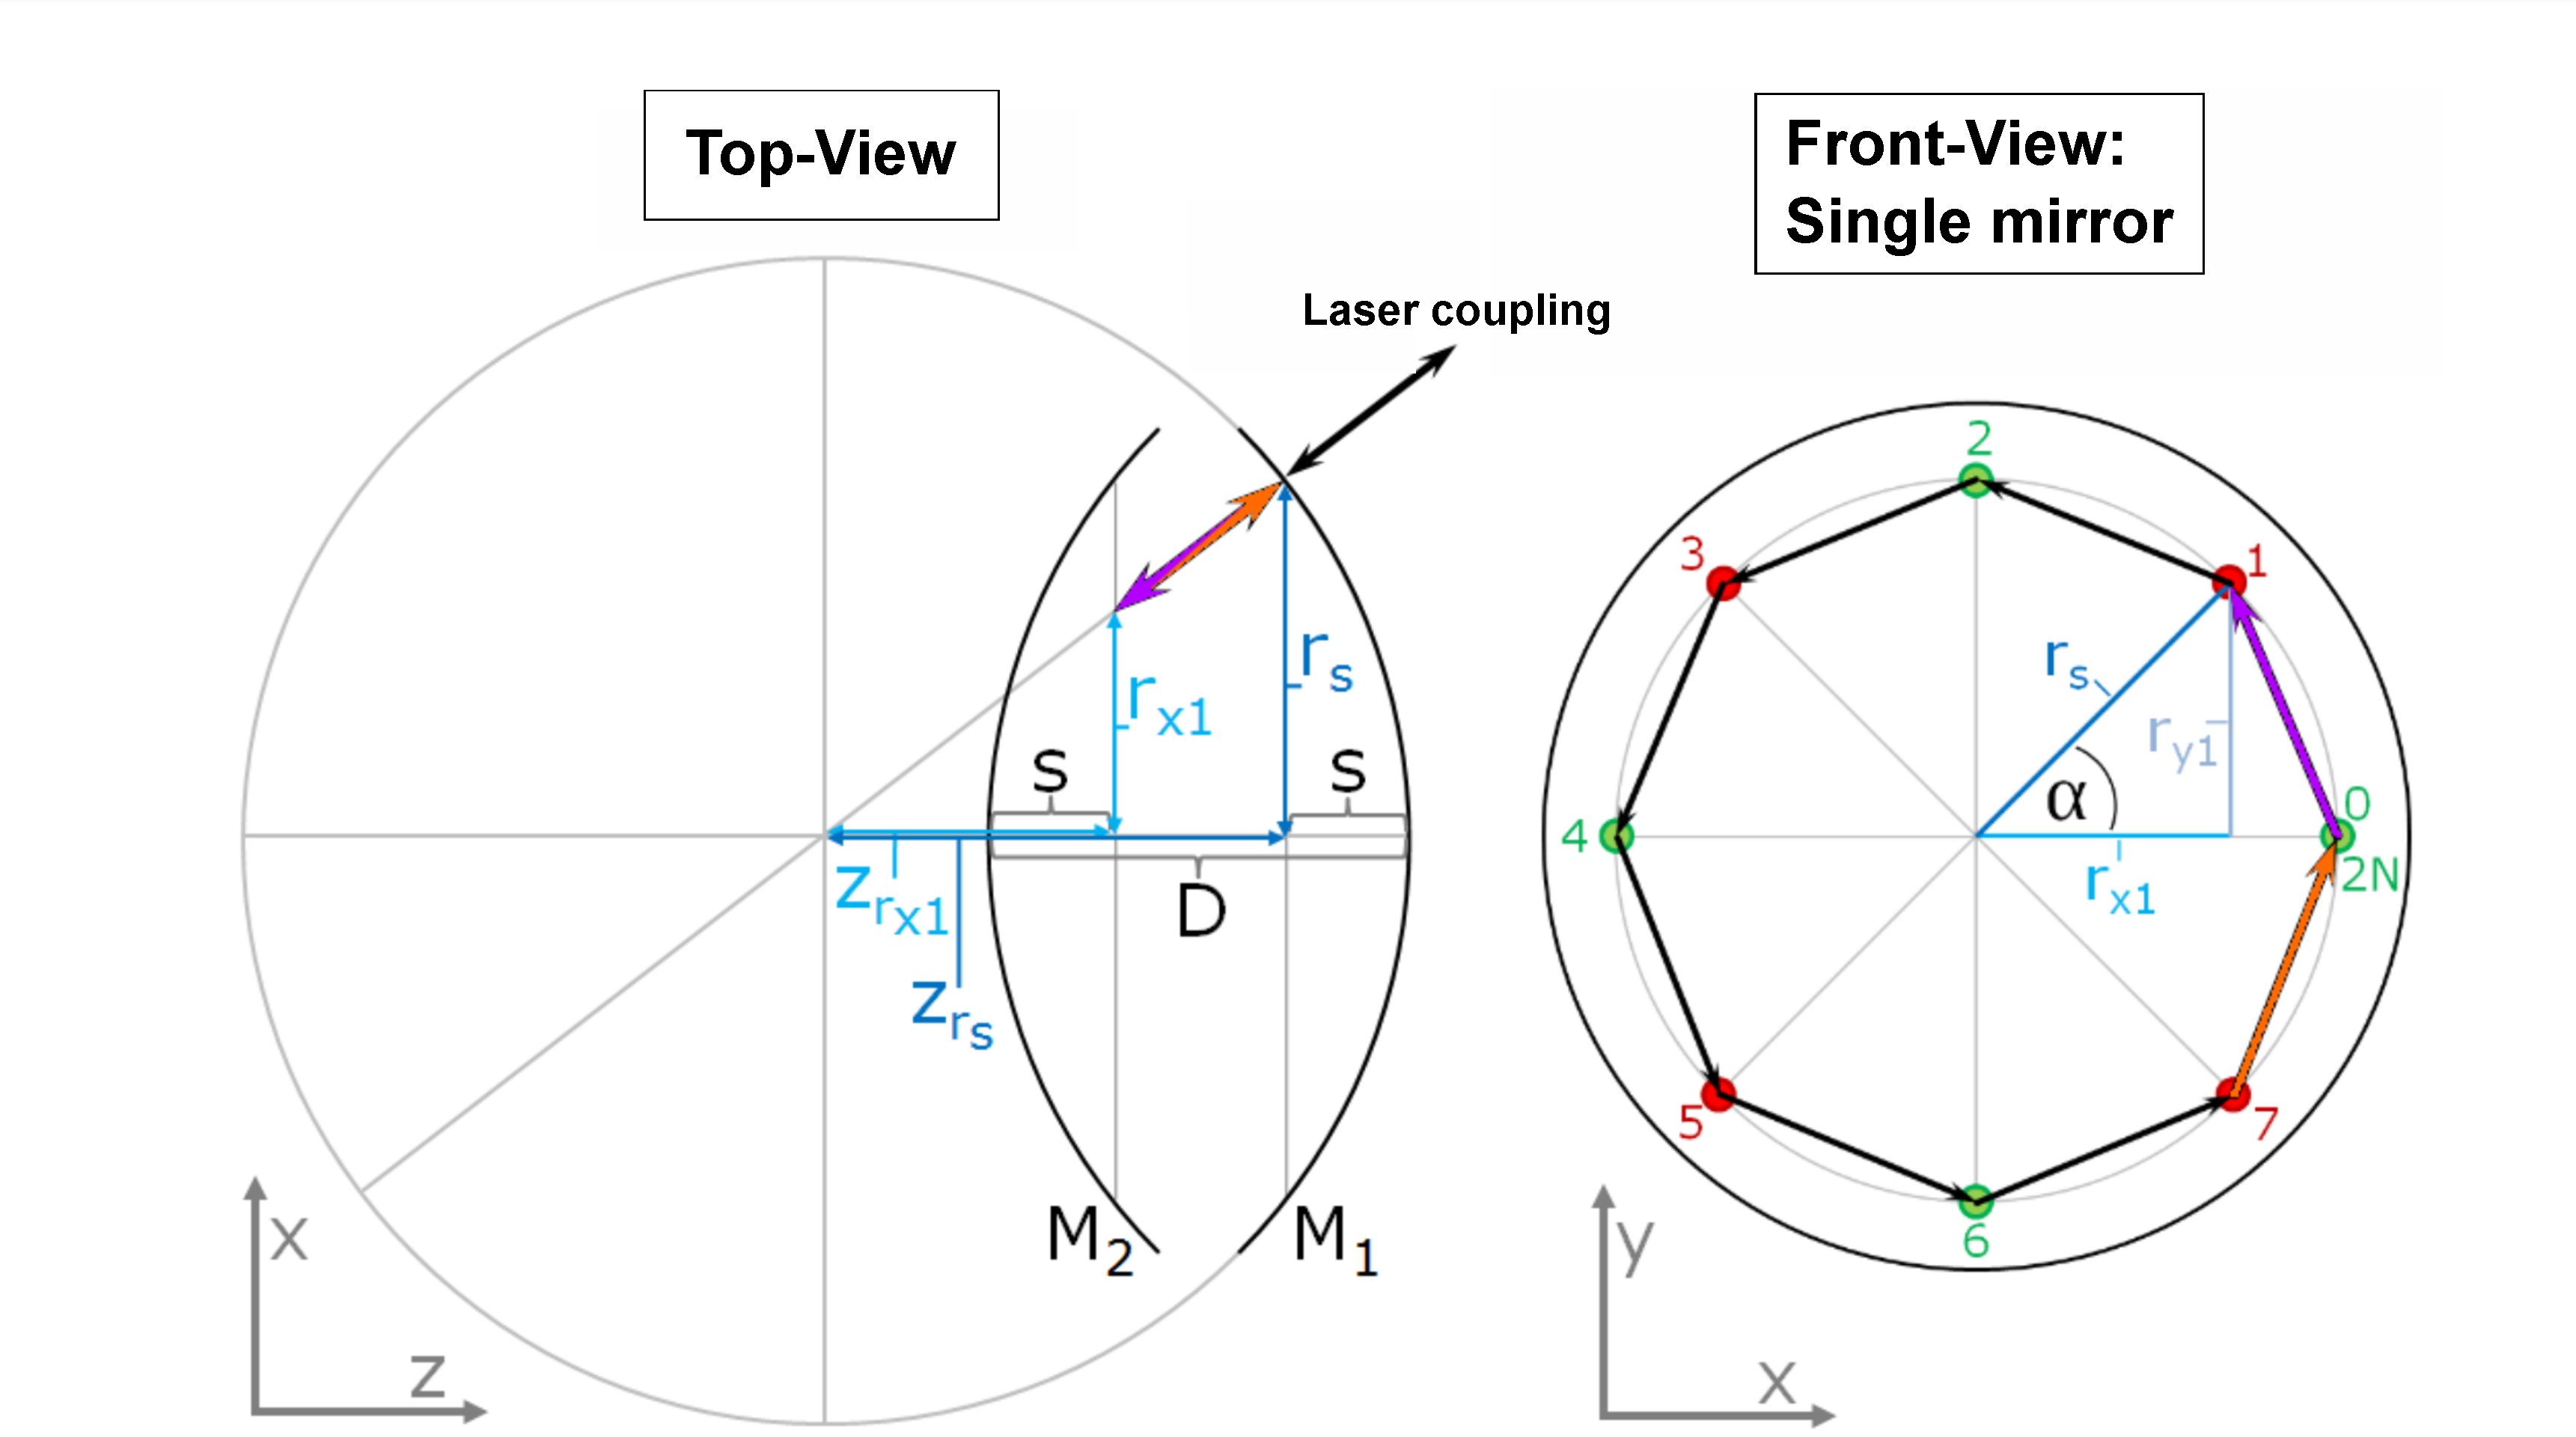
\includegraphics[width=\textwidth]{/Herriott-cell/Heriott-Cell-geometry}
	\caption{Shown on the left is the geometrical Top-view of a exemplaric Herriott-Cell configuration with a spherical spot pattern. On the right is the Front-view illustrating the directional change of the Laser beam after each reflection on the two mirrors.}
	\label{Figure:Heriott-cell-geometry}
\end{figure}
\noindent
The projection of the in- and out-coupled beam onto the x-z axis (Top-view in\ref{Figure:Heriott-cell-geometry}) shows, that for a spherical spot pattern, the respective beams must be overlapping in the respective plane. Assuming that the final beam is reflected on the mirror surface instead of leaving the cell through the hole, it would have to be reflected perpendicularly on the mirror surface to "re-enter" the Herriott Cell as the orange Laser Beam. Meaning that the in-coupled Laser beam always points to the center of the sphere or rather to the center of origin of the chosen coordinate system. This remains true even if the distance between the mirrors $D$ is increased or decreased and results in an characteristic property of Herriott-Cells: for a spherical spot pattern one has to re-align only the y-component of the in-coupled beam, when the mirror distance is changed. Using this information one can calculate $r_{x1}$  with the intercept theorem:
\begin{align}
	\frac{r_{x1}}{r_s}=	\frac{z_{rx1}}{z_{r_s}}
	\label{eq:Herriott-Cell-1}
\end{align}
where $z_{rx1}$ is the end position of the in-coupled, "purple" laser beam on the mirror without a hole and $z_{r_s}$ is the end position of the out-coupled, "orange" Laser beam on the mirror with the small hole. One can observe that:
\begin{align}
	z_{rx1}= R -D +s \ \ \text{   and } \ \ z_{r_s} = R-s
\end{align}
where $s$ is the spatial depths of the mirror which depends on its radius of curvature and the spot pattern:
\begin{align}
	s = R-\sqrt{R^2-r_s^2}
\end{align}
Equation \ref{eq:Herriott-Cell-1} can then be rewritten as:
\begin{align}
\begin{split}
	\frac{r_{x1}}{r_s}&=	\frac{R-D+s}{R-s}\\
	&= \frac{R-s+2s-D}{R-s}\\
	&=1 + \frac{2s-D}{R-s}
	\label{eq:Herriott-Cell-2}
\end{split}
\end{align}
Going back to the front view of figure \ref{Figure:Heriott-cell-geometry} one can see that for a closed, spherical configuration the 
angle $\alpha$ has to add up for each consecutive reflection, so that:
\begin{align}
	2N\alpha=2\pi \ \ \ \text{and} \ \ \ \cos{\alpha}=\frac{r_{x1}}{r_s}
	\label{eq:Herriott-Cell-3}
\end{align}
if the aforementioned condition was not true, the Laser beam would not be able leave the Herriott-Cell after one roundtrip (U=1 or 2N reflections for the example shown in figure\ref{Figure:Heriott-cell-geometry}). Using eq.\ref{eq:Herriott-Cell-3} to rewrite \ref{eq:Herriott-Cell-2} one obtains the mirror distance D as follows:
\begin{align}
	\cos{\alpha} &=	\frac{R-D+s}{R-s}\\
	D &= (R-s)(1-\cos{\alpha}) +2s
\end{align}
For a spherical spot pattern of the Herriott-Cell, the reflected Laser beams all travel an identical path between the two mirrors. The total optical path length can therefore be determined by summing over all single passes within the Cell. For one roundtrip U=1 with 2N reflections the total optical path length is given as:
\begin{align}
	L= 2N\cdot L_{single pass}
\end{align}
The geometrical pathlength of $L_{single pass}$ is:
\begin{align}
	L_{single pass} = \sqrt{\Delta x^2+\Delta y^2+\Delta z^2s}
\end{align}
where the respective Cartesian components can be determined with the help of figure\ref{Figure:Heriott-cell-geometry}.
\begin{align}
	\begin{split}
		\Delta x &=  r_s \cdot (1-\cos{\alpha})\\
		\Delta y &=  r_s \cdot \sin{\alpha}\\
		\Delta z &= D-2s = \sqrt{R^2-r_s^2}\cdot (1-\cos{\alpha})
	\end{split}
\end{align}
so that $L_{singlepass}$ can be rewritten as:
\begin{align}
\begin{split}
	L_{single pass} &= \sqrt{[r_s \cdot (1-\cos{\alpha})]^2+[r_s \cdot \sin{\alpha}]^2+[\sqrt{R^2-r_s^2}\cdot (1-\cos{\alpha})]^2}\\
	&= \sqrt{2r_s^2\cdot(1-\cos{\alpha})+(R^2-r_s^2)\cdot(1-\cos{\alpha})^2} \\
	&= \sqrt{2r_s^2\cdot(1-\cos{(\pi\frac{U}{N})})+(R^2-r_s^2)\cdot(1-\cos{(\pi\frac{U}{N})})^2}
\end{split}	
\end{align}
the overall optical path length $l$ then becomes:
\begin{align}
	l= 2N\cdot \sqrt{2r_s^2\cdot(1-\cos{(\pi\frac{U}{N})})+(R^2-r_s^2)\cdot(1-\cos{(\pi\frac{U}{N})})^2}
\end{align}

\section{Quantum cascade lasers}
Quantum cascade Lasers were theoretically predicted in the 1960s and experimental realized in 1994 by J.Faist et al \parencite{Faist1994}. Due to their working principle and gain material composition these semiconductor lasers can emit Laser light in a vast majority of the infrared- and terahertz-region of the electromagnetic spectrum. Since many molecules have absorbtion lines in these regions of the spectrum, quantum cascade Lasers have become the state-of-the-art light source for many spectroscopic applications.\\ \\ 
The working principle of a quantum cascade Laser is based on the quantum confinement of electrons in the conduction band of a semiconductor super lattice.
The required quantum well can be created by placing a thin layer of a material with a lower band-gap between two sheets of a semiconductor material with a high band-gap (e.g by using GaAs and GaAlAs). This quantum well confines the movement of the electrons along the surface normal of the sheets (z-direction). The layer thickness of the materials is generally in the order of a few nanometres (or less) and one can assume a one dimensional potential well to solve the corresponding Schrödinger equation and determine the energy eigenvalue of the quantum well:
\begin{equation}
(\mathcal{H}_{e}(\textbf{r}) + V_{con}(z))\Psi(\textbf{r}) = E\Psi(\textbf{r})
\label{Schroedinger-equation-quantum-well}
\end{equation}
with the confinement potential for an infinitely high well:

\[ V_{con}(z) =  \left\{
\begin{array}{ll}
0  & \text{for } -\frac{L_c}{2}< z < \frac{L_c}{2} \\
\infty & \text{for } |z| > \frac{L_c}{2}
\end{array} 
\right. \]
where $L_c$ is the width of the quantum well in the z-direction. The potential is symmetric around z=0 and one one can seperate the solutions for the spatial wave functions and energy eigenvalues into odd and even states. The  energy eigenvalues are given by:
\begin{align}
	E_{z,\text{even}} =& \frac{\hbar^2 \pi^2}{2m_e L_c^2} (2n-1)^2\nonumber\\
	E_{z,\text{odd}} =& \frac{\hbar^2 \pi^2}{2m_e L_c^2} (2n)^2, \text{ for }  n = 0,1,2,...
	\label{Schroedinger-equation-quantum-well-1}
\end{align}
The results show that the electrons have quantized eigenvalues within the valence and conduction band of the semiconductor and the energy of the states depends on the widths ($L_c$) of the sandwiched semiconductor sheet. One can further generalize the results of \ref{Schroedinger-equation-quantum-well-1} by adding the energy of the motion perpendicular to the z-direction. The total energy then becomes:


\begin{equation}
	E = \frac{\hbar^2}{2m_e}\left(\frac{n^2\pi^2}{L_c^2}+ k^2_{\perp}\right), \text{ for }  n = 0,1,2,...
	\label{Schroedinger-equation-quantum-well-energy-eigenvalues-2}
\end{equation}
It follows that the quantum confinement along the z-direction creates several equally spaced semiconductor sub-bands which are separated by $\frac{\hbar^2\pi^2}{2m_e L^2_c}$. (More realistic cases, for finite quantum wells, are showcased in \cite{Haug2009}). Radiative and non radiative transitions between these sub-bands of the semiconductor are called intersubband transitions. The intersubband transition energy can be altered by adjusting the width (L$_c$) of the sandwiched semiconductor materials. Fig. \ref{figure:QCL-dispersion-relation} illustrates the differences between intersubband transitions, which are used to drive QCLs and interband transitions which are the underlying principle of arbitrary laser diodes. 
\newpage
\begin{figure}[ht]
	\centering
	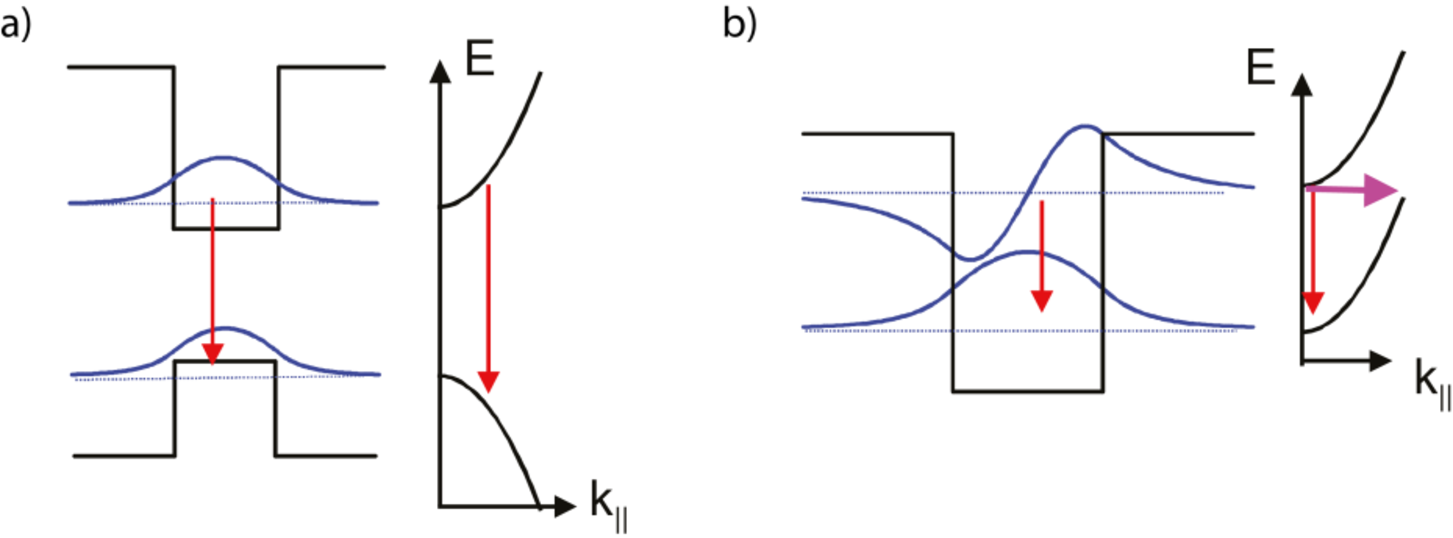
\includegraphics[width=0.75\textwidth]{/QuantumCascadeLasers/Disperion_relation_QCL}
	\caption{Conceptional difference between interband (a) and intersubband transitions (b). Interband transitions occur between the inversely shaped conduction and valence band. Intersubband transitions on the other hand appear between the (almost) parallel subbands of the conduction band of the semiconductor. The curvature of the bands also influences the gain of the respective lasers. Parallel bands result in a narrow, almost delta shaped, gain function while the gain of traditional interband lasers is step shaped due to the inverse curvature of the conduction and valence band. Image taken from: \cite{Faist2018}}
	\label{figure:QCL-dispersion-relation}
\end{figure}

\noindent  By clever engineering one can use the sub bands to create an effective four level laser system within the conduction band of a semiconductor super lattice. Generally, three quantum wells are combined with an injection and a relaxation area which together form one of the many unit cells of a QCL. While the quantum wells provide the three required energy levels of the Laser system, the injection area supplies the system with the necessary electrons and the relaxation depopulates the lowest energy level after the laser transition is complete.\\ \\ 
\noindent To create a population inversion between laser levels, electron tunneling from the injection area into a quantum well and from a well into the relaxation area is used. The tunneling speeds can be engineered to be much faster than depopulating effects, like elastic or inelastic scattering, occur. This results in a constant population of the highest energy level of the unit cell, while simultaneously the electrons from the lowest energy level are depopulated quickly.\\\\ 
Fig. \ref{figure:QCL-periodic-scheme} shows an exemplaric QCL heterostucture where a population inversion between the energy levels three and two is achieved by minimizing the spatial overlap of the two states. This can be achieved by adjusting the width of the quantum wells as well as the semiconductor barriers that separate them. The transition time $\tau_{32}$ therefore becomes around one order of magnitude slower than the depopulation rate $\tau_{2}$ and the condition for a population inversion $\tau_{32}>\tau_{2}$ is fulfilled. By applying a bias voltage along the z-axis of the semiconductor super lattice, the potential gets the characteristic stair-case-shape and allows the electrons to cascade through multiple unit cells. 
\begin{figure}[H]
	\centering
	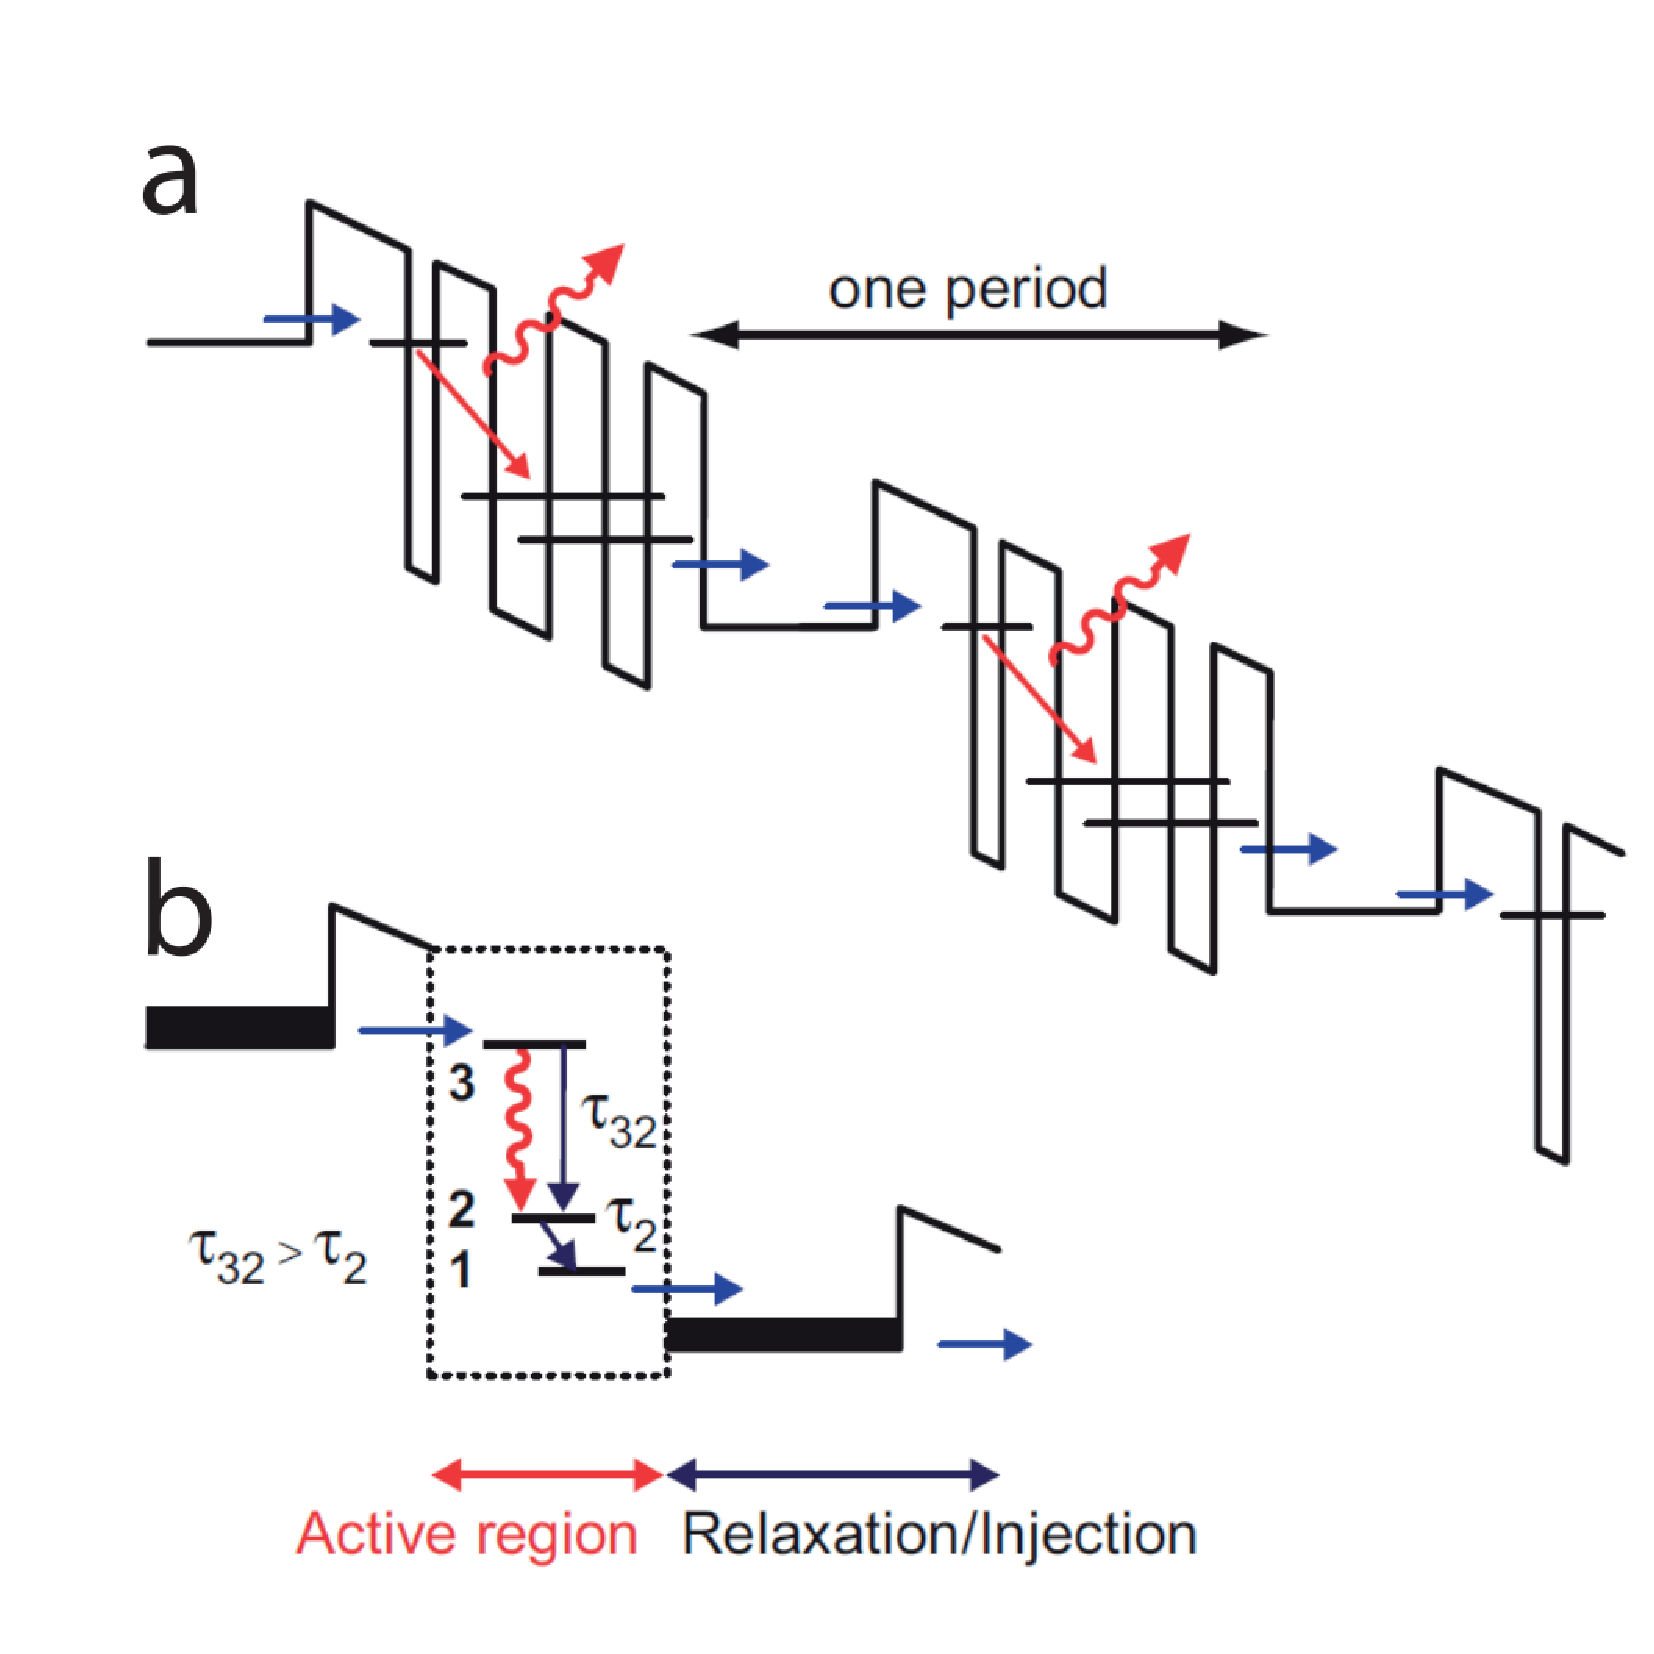
\includegraphics[width=0.75\textwidth]{/QuantumCascadeLasers/QCL_Periodic_Scheme}
	\caption{a) Periodic structure of a Quantum cascade Laser. b) Simplified unit cell of a QCL, containing all relevant energy levels and transition times. Source: \cite{Faist2018}}
	\label{figure:QCL-periodic-scheme}
\end{figure}
\newpage
\chapter{Theory part II: Refractometry}
\section{Ideal and real gases}
With the redefinition of the SI-system in 2019, gas density measurements became an interesting contestor to classical pressure assessments via measurements of the mechanical force that is acting on a surface area.  Important natural constants like the Boltzmann constant k$_b$, the Avogadro constant N$_a$ and the gas constant R were assigned uncertainties of zero after the redefinition. Which makes the ideal gas law:
\begin{align}
	p&=\rho_N k_B T \text{, with  } \rho_N=\frac{vN_a}{V} \nonumber\\
	p&=\rho_v R T \text{, with  } R=k_bN_a
	\label{eq:ideal_gas_law}
\end{align}
an appealing foundation for the construction of density based pressure-standards for the vacuum region, which are also traceable as long as the density $\rho$ can be assessed in a traceable manner.\\\\
\noindent
The ideal gas law eq.:\ref{eq:ideal_gas_law} is a simplistic approach, that does not account for electromagnetic particle-particle interactions (e.g van der Waals forces) or quadratic long-range interactions \cite{Jousten-2017}, which both depend on the particle density. By expanding the ideal gas law in a Taylor series for $\rho_v$ one can account for additional density dependent effects and obtains the real gas law:
\begin{align}
	p=\rho_v R T (1+ B(T) \rho_v + C(T)\rho_v^2 + ...)
	\label{eq:real_gas_law}
\end{align}
with the second and third density virial coefficients B(T) and C(T). The higher order virial coefficients account for multi molecule collisions, which are unlikely to occur in the vacuum regime and are therefore often times neglected for said pressure region. Figure\ref{figure:density_virials} illustrates the relation between the gas density and the partial pressure of Nitrogen for a fixed temperature of \mbox{300 K}. The difference between the real and ideal Nitrogen gas is shown by the residuals from the upper plot. At atmospheric pressure the difference between the two is around \mbox{200 ppm}. For pressures above 10$^6$ Pa (10 Bar), the influence of the quadratic third virial coefficient is clearly visible. The respective values for the second and third density virials were taken from: \cite{Sevast-1986}.
\begin{figure}[ht]
	\centering
	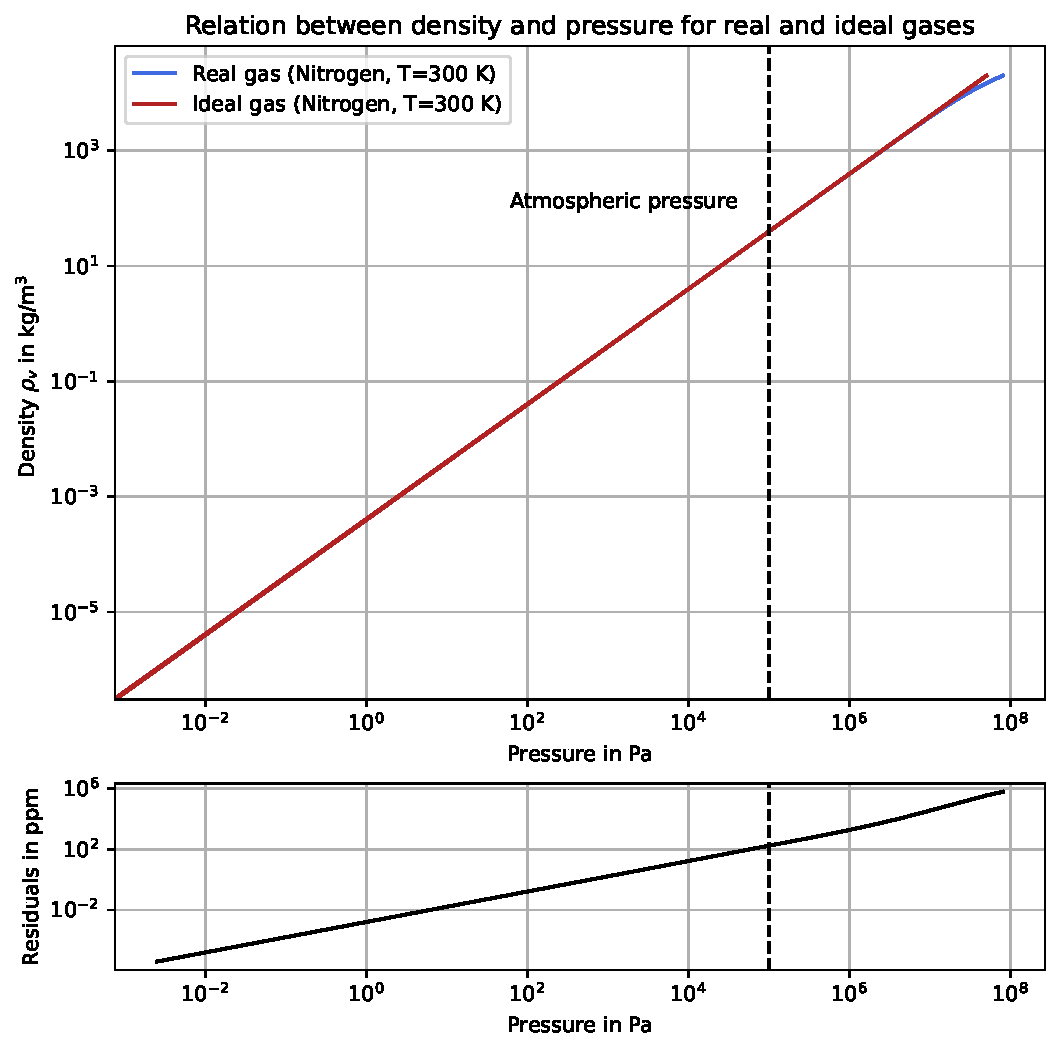
\includegraphics[width=0.9\textwidth]{FPI-Theory/Density_virials_Nitrogen_300K}
	\caption{Top: Comparison between ideal and real Nitrogen gas at 300 K.\\
				Bottom:  Residuals between the ideal and real Nitrogen gas.}
	\label{figure:density_virials}
\end{figure}
\newpage
\section{Lorentz Lorenz equation}
If light travels through a gaseous medium it can be absorbed or dispersed. In the case of absorption the light is in resonance with an electromagnetic transition of an atom or molecule and the respective photon energy is transferred to the molecule. In the case of dispersion the molecules are polarized and start oscillating at a frequency similar to that of the photon \cite{Jousten-2017}. This results in net reduction of the traveling speed of the photon which can be described by the frequency dependent refractive index n$(\nu)$ of the gas:
\begin{align}
	c=\frac{c_0}{n(\nu)}
	\label{eq:refractive_index}
\end{align} 
where c$_0$ is the speed of light in vacuum. The electric polarizability of a gas describes how susceptible a molecule or atom is to have a dipole moment induced by an external electrical- or photon-field. For a gaseous medium, every molecule has its own internal electrical field and is furthermore exposed to the electric fields of the surrounding molecules and any additional external field, which can modify the internal state of the molecules. The properties of the matter can then be determined by averaging over all the electrical fields within it. The Lorentz-Lorenz equation relates the polarizability with the refractive index of gas and a detailed field-theory based derivation is given in \cite{Born-1980}. The Lorentz-Lorenz equation is given as:
\begin{align}
	\frac{\alpha}{3 \epsilon_0}\rho_N=\frac{N_A\alpha}{3 \epsilon_0}\rho_v=A_R\rho_v=\frac{n^2-1}{n^2+2}
	\label{eg:Lorentz-Lorenz}
\end{align}
With the dynamic polarizability $\alpha$, the dynamic molar polarizability $A_R$ and the absolute dielectric permittivity in vacuum $\epsilon_0$. The Lorentz-Lorenz equation does not include magnetic effects on the gas  molecules nor the inter molecular effects that the gas molecules have on each other. The inter molecular effects again depend on the gas density and can be including by expanding equation \ref{eg:Lorentz-Lorenz} in a Taylor series for $\rho_v$:
\begin{align}
	\frac{n^2-1}{n^2+2}=A_R\rho_v(1+b_R(T)\rho_v+c_R(T)\rho_v^2+...)
	\label{eg:Lorentz-Lorenz_1}
\end{align}
where $b_R$ and $c_R$ are the second and third, temperature dependent, refractivity virial coefficients.\\\\
\noindent
For gases and wavelengths in the visible spectrum, the refractive index n is generally close to 1 (n = 1.000282 for nitrogen at 15$^{\circ}$C and $\nu= 627$ nm,\cite{Peck-1966}). Knowing this, one can use the two simplifications:
\begin{align}
	n^2-1 \approx  2(n-1) \text{ and } n^2+2 \approx 3
	\label{eg:Lorentz-Lorenz_simplification}
\end{align}
to approximate the Lorentz-Lorenz equation (\ref{eg:Lorentz-Lorenz}) to:
\begin{align}
	n-1 \approx \frac{\alpha}{2\epsilon_0}\rho_N
	\label{eg:Lorentz-Lorenz_approximated}
\end{align}
which directly relates the gas density $\rho_N$ to the refractivity n-1 of the gas.
\section{Refractometry}
Since both, the Lorentz-Lorenz equation and the real gas law, depend on the gas density one can combine the two equations to derive a protocol to measure the pressure P as a function of the frequency dependent refractivity: n($\nu$)-1. Devices that utilize this relationship between the two properties are called refractometers. \\\\
\noindent
One approach to measure the refractive index of a gas is to use Fabry-Pérot cavities. The resonator can be filled with a gas at a fixed pressure P and the resonance frequencies of the Fabry-Pérot can be compared for the evacuated and gas-filled state of the system. For a simplistic, non-deformable cavity following the methodology presented in \cite{Jousten-2017}, one would obtain the latter experimental property:
\begin{align}
	\mu_{\kappa=0}=\frac{(\frac{\nu_0}{\nu_P})^2-1}{(\frac{\nu_0}{\nu_p})^2+2}
	\label{eg:refractrometry_measurement_prperty}
\end{align}
where $\kappa=0$ is the assumed zero compressibility of the cavity material, $\nu_0$ is the resonance frequency of the FP-cavity in an evacuated state and $\nu_P$ is the resonance frequency of the FP-cavity in the gas-filled state.\\\\
\noindent
Combining the real gas law (equation \ref{eq:real_gas_law}) with the Lorentz-Lorenz equation (\ref{eg:Lorentz-Lorenz_1}) then yields an experimental approach to realize a refractometry based pressure standard:
\begin{align}
	P=\frac{RT}{A_R}\left(\mu_{\kappa=0}+\mu_{\kappa=0}^2\frac{(B-b_R)}{A_R}+\mu_{\kappa=0}^3\frac{C-2Bb_R+2b{_R}^2-c_R}{A{_R}^2}+...\right)
	\label{eg:experimental_formular_refractometry}
\end{align}
However, the pressure induced deformation of the resonator length can not be ignored if the lowest measurement uncertainties are desired. For a linear, homogeneous deformation of the resonator, with $\kappa >0$, one can describe the pressure induced length change of the resonator as:
\begin{align}
	l_P=l_0+l_0\kappa P \leftrightarrow \frac{l_P}{l_0}=1+\kappa P
	\label{eg:refractometer_length_change}
\end{align}
where $l_P$ and $l_0$ are the resonator lengths with and without an applied gas pressure P respectively and $\kappa$ is the effective length compressibility. Equation \ref{eg:refractrometry_measurement_prperty} can then be reworked to also account for the deformation of the system:
\begin{align}
	\mu_{\kappa}=\frac{(\frac{\nu_0}{\nu_P})^2-1}{(\frac{\nu_0}{\nu_p})^2+2}=\frac{n^2\cdot(1+\kappa P)^2 -1}{n^2\cdot(1+\kappa P)^2 +2} \approx \frac{n^2\cdot(1+2\kappa P) -1}{n^2\cdot(1+2\kappa P) +2}
	\label{eg:refractrometry_measurement_prperty_with_deformation}
\end{align}
In the last step quadratic terms in $\kappa$ were discarded since the compressibility for glasses (e.g Quartz glass: $\kappa \approx 2.7 \cdot 10^{-10}$ m/Pa ) is very small. The working equation for the refractometry based pressure standard then becomes:
\begin{align}
	P=\frac{RT}{A_R+\frac{2\kappa RT}{3}}\left(\mu_{\kappa}+\mu_{\kappa}^2\frac{(B-b_R-\frac{2\kappa RT}{3})}{A_R+\frac{2\kappa RT}{3}}+...\right)
	\label{eg:experimental_formular_refractometry_kength_corrected}
\end{align}
after combining equations \ref{eg:refractrometry_measurement_prperty_with_deformation}, \ref{eq:real_gas_law}) and \ref{eg:Lorentz-Lorenz_1} up to the second order of the Taylor expansions.
\subsection{Dual Farby-Pérot cavity based refractometry}
For experimental dual-FPC based approaches to refractometry it is convenient to measure the refractivity n-1 of the investigated gas, based on a shift to a beat measurement $\frac{\Delta f}{\nu_0}$ instead of two individual Laser frequency measurements. This has practical reasons, since beat frequencies, up to several GHz, can be measured and evaluated with relatively cheap equipment like high-speed beat detectors, frequency counters and spectrum analyzers. State of the art RF-electronics can also be read at a high speed and basically allow for real-time investigations of the chosen system.\\\\
The beat frequency $\Delta f$ between the two lasers, which are phase locked to the resonance frequencies of the respective measurement and evacuated reference FP-cavity, shifts if additional gas is introduced or removed from one of the FP-cavities. When mode jumps take place, the mode number $\Delta q$ has to be adjusted accordingly and one can
assess the refractivity of the investigated gas as a function of the change in beat frequency between the two laser fields:
\begin{align}
	n-1=\frac{\Delta f +\Delta q_m}{1-\delta f +\epsilon_m}
	\label{eg:}
\end{align}
\chapter{Theory part III: Optical resonators}
\section{Fabry-Pérot resonators}
A Fabry-Pérot interferometer (FPI) is a basic optical resonator that consist of two plan-parallel mirrors which are often times attached to a deformation resistant spacer material with a constant length L. FPI's are commonly used for high resolution spectroscopy or as Laser resonators. The incident light is reflected between the two highly reflective mirrors, which results in multi-beam interference inside the resonator. The interference is constructive when the resonance condition is met and the longitudinal resonator modes (frequencies at which constructive interference is possible) are given as:
\begin{equation}
	\nu_q = \frac{qc}{2nL}
	\label{resonacne_condition_FPI}
\end{equation}
where q is the (integer) mode number,  c is the speed of light, L the length of the cavity and n the refractive index of the gas inside the FPI. Only light with the the proper frequencies $\nu_q$ is transmitted through the resonator which makes FPI's great optical filters. The quality of this filter is described by the free spectral range (FSR) and the finesse of the resonator. The FSR is the frequency difference between two consecutive longitudinal resonator modes and is given by:
\begin{equation}
	\Delta \nu = \nu_{q_{i+1}} - \nu_{q_i} = \frac{c}{2nL}
	\label{Free_spectral_range_of_FPI}
\end{equation}
The finesse describes the spectral broadening of the resonator modes in relation to the free spectral range. The finesse correlates directly with the reflectivity of the mirrors and is given by:
\begin{equation}
	F= \frac{\Delta \nu}{\nu_{\scriptscriptstyle FWHM}} =\frac{ \pi \sqrt{r}}{1 - r}
	\label{Finesse_of_FPI}
\end{equation}
\subsection{Longitudinal resonator modes}
If the multiple reflection of a plane wave between two plane-parallel partially reflecting layers is considered, the finesse and the free spectral range can be derived directly from wave theory. The incident wave: 
\begin{equation}
	E=E_0 e^{i(\omega t - kx)}
	\label{wave_eqaution_FPI}
\end{equation}
hits the reflecting surfaces at an angle $\alpha =0$ and is split into two partial beams at each mirror. One partial beam is reflected and one is transmitted through the mirror (see figure \ref{figure:FPI-wave_theory}).  The initial partial Beam $E_1$ transmitted through the FPI experienced no reflections inside the resonator but was transmitted through both mirrors. Its amplitude is therefore given by 
\begin{align*}
	E_1= E_0 t^2 e^{ikL} 
\end{align*}
where t is the transmittance of the mirror given by $t=\frac{E_t}{E_0}$. Due to the finite distance L between the two mirrors, each round-trip of the partial wave inside the cavity accumulates an additional phase $e^{i\delta} $ with $\delta = 2kL$. The second partial beam ($E_2$) that is transmitted through the FPI has experienced two transmission and two reflections. Its amplitude can again be written as: 
\begin{equation*}
	E_2= E_0 t^2e^{i\frac{\delta}{2}} r^2 e^{i\delta}
\end{equation*}
with the similarly defined mirror reflectance $r=\frac{E_r}{E_0}$. 
\begin{figure}[ht]
	\centering
	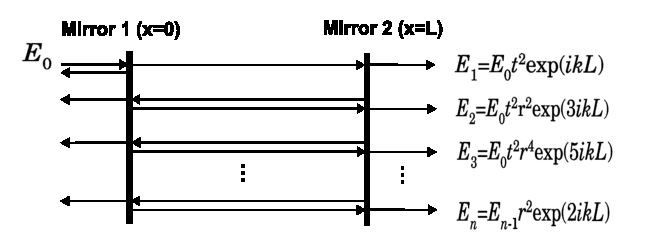
\includegraphics[width=0.9\textwidth]{FPI-Theory/FPI_mirrors_wave_theory}
	\caption{Illustrated are the reflections and transmissions of a simple FPI. Image taken and reworked from: \cite{Lauterborn2003}}
	\label{figure:FPI-wave_theory}
\end{figure}
\\ \\ \noindent
For many spectroscopic applications the light that is transmitted through the resonator is of greatest interest, since it represents the frequencies of the light that can freely path through the optical filter (longitudinal resonator modes). Summing over all partial waves, including the correct phase shift, yields the total transmitted amplitude \cite{DemtroederLaser2011}\cite{Lauterborn2003}.
\begin{equation*}
	E_t = \sum_{n=1}^{\infty} E_n = E_0 t^2 e^{i\frac{\delta}{2}} \sum_{n=1}^{\infty} r^{2(n-1)}e^{i\delta(n-1)}= E_0t^2e^{i\frac{\delta}{2}}\sum_{n=0}^{\infty}\left(r^2 e^{i\delta} \right)^n
\end{equation*}
This geometrical sum can be written in closed form as:
\begin{equation}
	E_t = \frac{E_0 t^2 e^{i\frac{\delta}{2}}}{1-r^2e^{i\delta}}
	\label{FPI_wave_amplitudes_trans_total}
\end{equation}
The corresponding transmitted total intensity is given by the Airy function as following:
\begin{align}
	\begin{split}
		I_t&= E_tE_t^*= E_0E_0^* t^4 \frac{1}{(1-r^2e^{i\delta})(1-r^2e^{-i\delta})}\\
		&=I_0 t^4 \frac{1}{1+r^4-2r^2\cos(\delta)}\\
		&=\frac{I_0}{1+\left(\frac{2r}{1-r^2}\right)^2\sin^2(\frac{\delta}{2})} = \frac{I_0}{1+F^*\cdot\sin^2(\frac{\delta}{2})}
		\label{eq:airy_function}
	\end{split}
\end{align}
in the last step the trigonometric identity $\cos(2x)=1-\sin^2(x)$ was used together with the conservation of energy which states: $r^2+t^2=1$. The introduced factor $F^*=\left(\frac{2r}{1-r^2}\right)^2$ is the Finesse coefficient. Figure \ref{figure:FPI_aery_function} shows the Airy function for different resonator configurations. The points of greatest interest are the maxima at which all light is transmitted through the cavity and the distance between the individual peaks which defines the FSR or the spectral resolution if the FPI is used as a spectrometer.
\begin{figure}[ht]
	\centering
	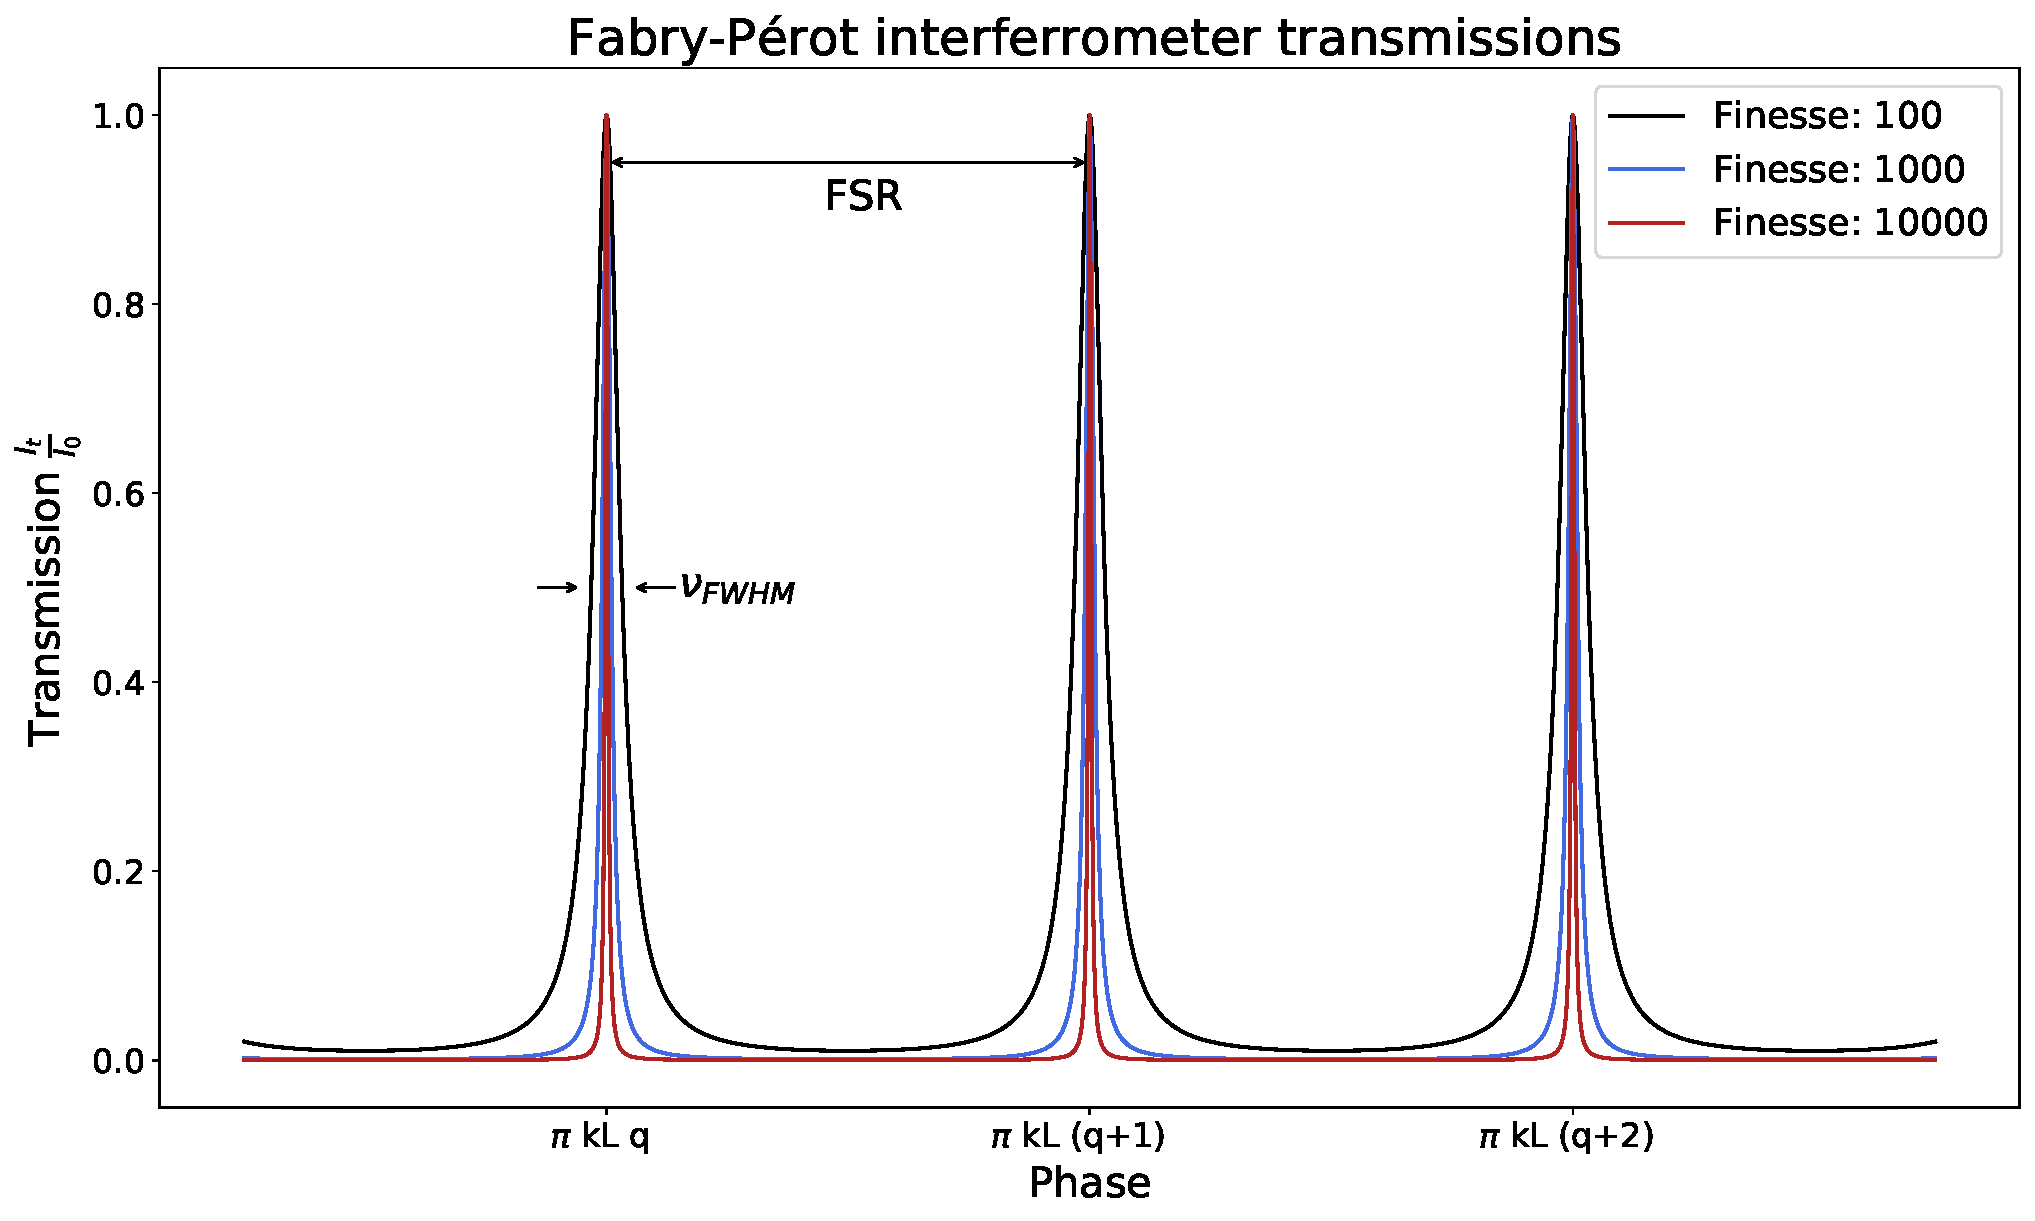
\includegraphics[width=0.9\textwidth]{FPI-Theory/Aery_function_FPI_modes}
	\caption{Shown are three different FPI resonator configurations with different values for their finesse and their respective longitudinal resonator modes.}
	\label{figure:FPI_aery_function}
\end{figure}\\\\ \noindent
Two consecutive waves with the wave vectors $k_q$ and $k_{q+1}$ have a phase difference of $\pi$. Using $\nu= \frac{c}{2\pi} k$ one can again calculate the FSR:
\begin{align}
	\begin{split}
		\pi &= (k_{q+1} - k_q)L  = \Delta k L\\
		&= \frac{2\pi \Delta \nu}{c}L \Rightarrow \Delta \nu = \frac{c}{2L}
		\label{eq:FSR_calculated}
	\end{split}
\end{align}
Using the definition of the finesse which is given as the ratio of the FSR to the frequency widths $\nu_{\scriptscriptstyle FWHM}$ of the resonator  modes at half their maximal Intensity, so $\frac{I_t}{I_0}=\frac{1}{2}$, one can derive an expression for the finesse directly from eq. \ref{eq:airy_function}:
\begin{align}
	\frac{1}{2} = \frac{1}{1+F^*\cdot \sin^2(k'L)} \text{     with      } F^*\cdot \sin^2(k'L) \overset{!}{=} 1
\end{align}
This can only be achieved for reasonably small wave vectors $k'$ and therefore large mirror reflectivities. For small $k'$ one can rewrite \cite{Lauterborn2003}:
\begin{align*}
	F^*\cdot \sin^2(k'L) \approx  F^*(k'L)^2 = F^*\left(\frac{\pi \nu_{\scriptscriptstyle FWHM}}{c} L\right)^2
\end{align*}
With the definition of the finesse coefficient $F^*$ introduced in \ref{eq:airy_function} one can derive an expression for the required frequency widths $\nu_{\scriptscriptstyle FWHM}$.
\begin{align}
	\nu_{\scriptscriptstyle FWHM}= \frac{c}{\sqrt{F^*}L\pi} = \frac{c(1-r^2)}{2rL\pi}
	\label{eq:f_FWHM_calculated}
\end{align}
The finesse $F$ can the be calculated with the results from eq.(\ref{eq:FSR_calculated}) and eq.(\ref{eq:f_FWHM_calculated}):
\begin{align}
	F=\frac{\Delta\nu}{\nu_{\scriptscriptstyle FWHM}}=\frac{r\pi}{1-r^2}
\end{align}
\subsection{Gaussian Beam propagation}
Due to their optical properties, Fabry-Pérot resonators are commonly used as a frequency reference for Laser systems. The Laser light (generally) has a Gaussian beam profile with varying coherence length, depending on the laser type used. In practice FPI's are therefore often realized with at least one spherical mirror which is used to refocus the light and greatly simplifies the optical alignment and stability of the cavity. To form a stable resonator the condition:
\begin{align}
	0\leq g_1g_2\leq 1
\end{align}
For the case $g_1g_2=1$ (plan-plan) the resonator is theoretically still stable but creates infinitely large beam spots at the mirrors which makes the configuration practically unstable.
The beams, reflected back and forth within these resonator types, retain their Gaussian profile. However, inherent properties such as the beam radius and the position of the beam waist are influenced by the mirrors curvature and have to be taken into account during optical alignment to ensure optimal coupling into the resonator. The beam radius $\omega(z)$ of the Gaussian beam, along the optical axis, is given by:
\begin{eqnarray}
	\omega(z)=\omega_0 \sqrt{1+(\frac{z}{z_R})^2} \text{\ \ \ with \ \ \ } z_R =\frac{\pi \omega_0^2}{\lambda}
	\label{eq:FPI_gaussian_spotsize} 
\end{eqnarray}
where $\omega_0$ is the beam waist and $z_R$ is the Rayleigh length. To couple light into a e.g confocal resonator efficiently, the beam profile outside and inside of the resonator have to match. In the case of the aforementioned confocal configuration this can be achieved by creating a focus of the Laser beam at $L/2$, the center of the cavity, which can be realized experimentally with a set of lenses.
\subsection{Transversal Resonator modes}
In addition to the Gaussian mode, higher-order transverse electromagnetic modes (TEM$_{mn}$) can also be formed inside the resonator. Their electrical field can described by the Hermite-Gauss polynomials ($H_n$, where n is the respective polynomial order) and is given by:
\begin{eqnarray}
	E_{mn}(x,y,z)=E_0\frac{\omega_0}{\omega(z)} H_m (\frac{\sqrt{2}x}{\omega(z)})H_n(\frac{\sqrt{2}y}{\omega(z)}) \\ \nonumber
	\cdot exp[-(x^2+y^2)(\frac{1}{\omega^2(z)}-\frac{ik}{2}R(z))+ikz-i(m+n+1)\tan^{-1}(\frac{z}{z_0})]
	\label{eq:FPI_transversal_modes_E_field} 
\end{eqnarray}
with the radius of curvature of the wavefront $R(z)= z+\frac{z_0^2}{z}$ and the transversal mode numbers $m$ an $n$. \\\\
The frequencies of the transversal modes are given as:
\begin{eqnarray}
	\nu_{qmn}= \frac{c}{2L} \left( q+ \frac{1}{\pi}(m+n+1)\cos^{-1}(\sqrt{g_1g_2}) \right )
	\label{eq:FPI_transversal_mode_frequencies} 
\end{eqnarray}
For $m=n=0$ one obtains the TEM$_{00}$ mode which is equivalent to the Gaussian mode. For experimental applications it is often times desirable to only excite the TEM$_{00}$ mode inside the resonator, since the overall transmitted intensity is highest and the Laser beam retains its optical properties. Figure \ref{figure:FPI_TEM_modes} shows the first 16 TEM modes, starting with the TEM$_{00}$ up to the TEM$_{33}$-mode. \\\\
\begin{figure}[ht]
	\centering
	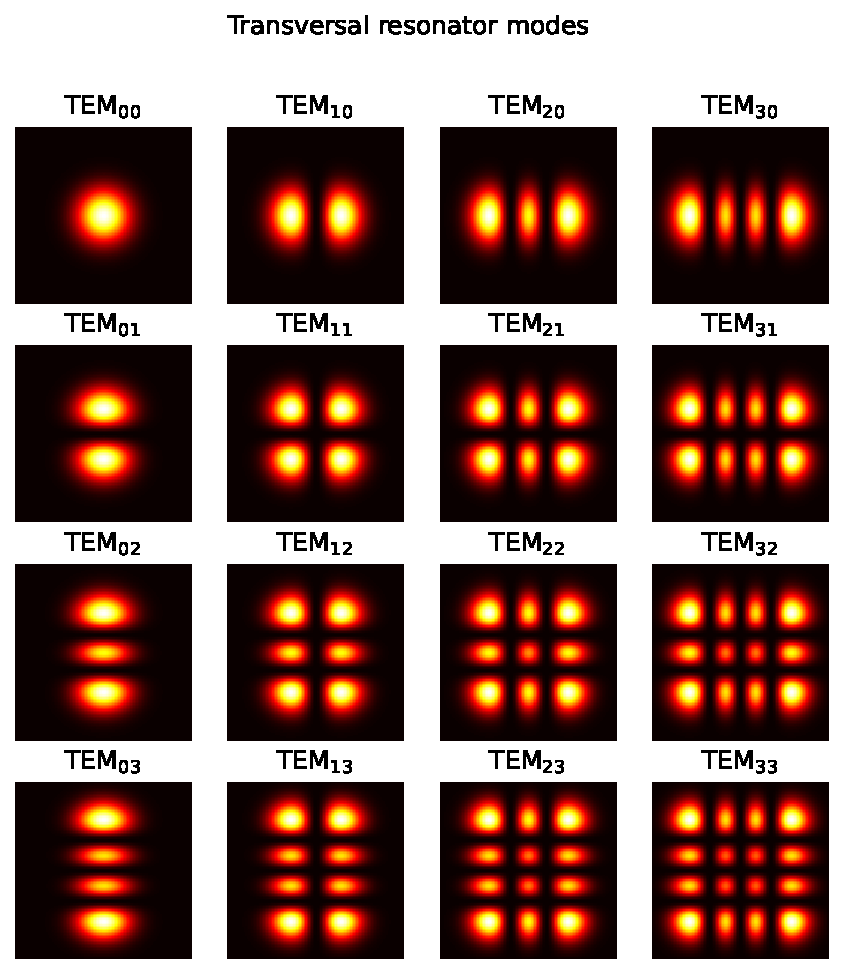
\includegraphics[width=0.7\textwidth]{FPI-Theory/TEM_modes}
	\caption{Shown are the first 16 TEM-modes. Starting from the TEM$_{00}$- and going up to the TEM$_{22}$-mode.}
	\label{figure:FPI_TEM_modes}
\end{figure}
\newpage
\noindent
\subsection{Mode-matching}
In the context of refractometry, it is often times important to only excite the TEM$_{00}$ with the chosen Laser source. This is required to correctly identify the Laser frequency and avoid complications with Laser-locking techniques. 
Higher order modes are generally only excited if the incident Laser beam spatially overlaps with them, which can be avoided by proper Laser alignment. If the beam propagation and spatial profile of the Laser light match with spatial profile of the TEM$_{00}$ inside the resonator, only the TEM$_{00}$ mode will be excited inside the cavity. With knowledge of the radius of curvature of the cavity mirrors, the mirror distance and cavity type (spherical-spherical or plan-spherical mirrors) one can ideally mode-match the Laser with the resonator.
Figure \ref{figure:FPI_mode_matching} illustrates the basic operating principle of spatial mode-matching.
\begin{figure}[H] 
	\centering
	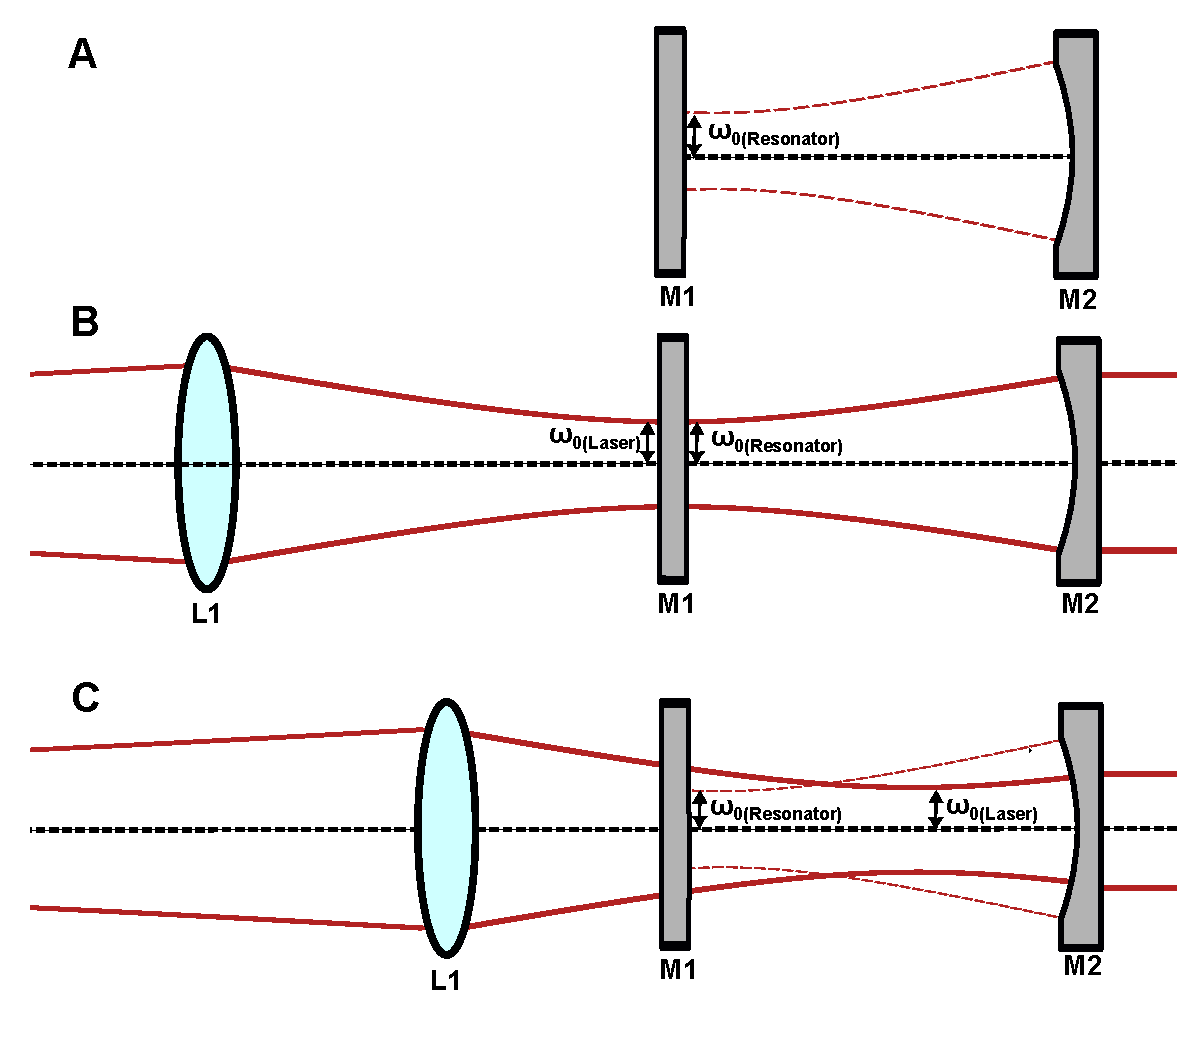
\includegraphics[width=0.95\textwidth]{FPI-Theory/Mode_Matching}
	\caption{\\A) Plan-spherical resonator shown together with the ideal Gaussian beam propagation.\\
		B) Mode matched Laser and resonator.\\
		C) Sub-par matching of the spatial profiles of the Laser and the resonator.}
	\label{figure:FPI_mode_matching}
\end{figure}
\newpage
\noindent
\textbf{Case A} shows the stable configuration for a TEM$_{00}$ mode in a plan-spherical resonator and the respective beam waist $\omega_0$(resonator), which is located at the planar mirror.\\\\
For \textbf{case B} a Laser together with a focusing lens L1 is added. The Laser is mode matched with the resonator for a properly chosen focusing lens. The beam waist of the Laser ($\omega_0$(Laser)) and the beam waist of the resonator are located at the same position along the propagation axis of the light.\\\\
\textbf{Case C} illustrated the sub-par matching of the Laser and the resonator. This configuration can results in less Laser light intensity being transmitted through the resonator and additional, unwanted resonator modes being excited inside the cavity.\\\\
\noindent
For invisible lasers, it is useful to look at the intensity transmitted through the resonator while the laser is de-tuned in frequency. The laser can then be adjusted so that only the longitudinal modes are visible in the spectrum. This can be achieved with a simple experimental setup, which only requires a photodetector, a Laser and the FPI. Figure \ref{figure:FPI_TEM_detector_spectrum} shows a simulated detector signal, which can be observed when the Laser is de-tuned in its frequency by applying a voltage ramp to the Laser-driver. The first spectrum is typical for a miss aligned Laser with respect to the cavity. The spectrum on the right shows the signal for a almost perfectly mode matched Laser. The TEM$_{00}$ modes have the highest possible intensity and no higher order modes are visible.\\\\
\begin{figure}[H]
	\centering
	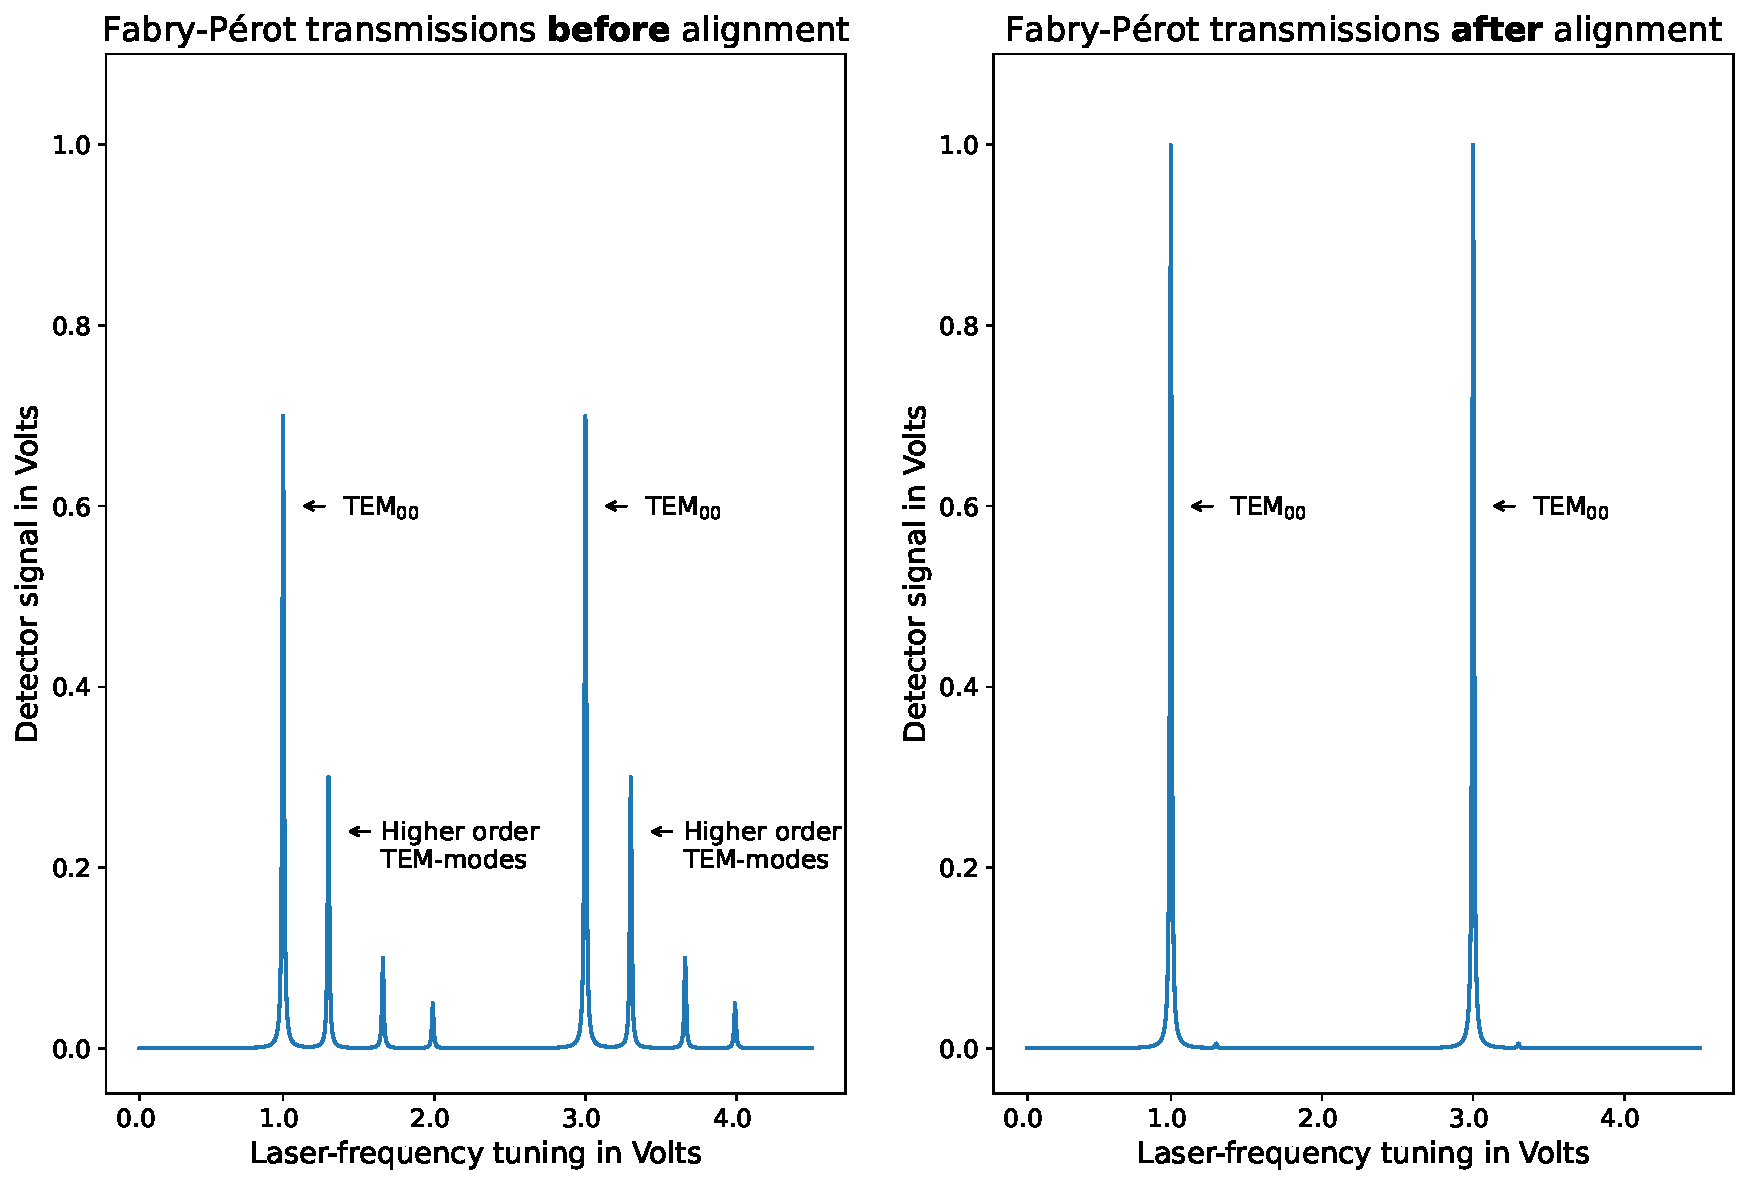
\includegraphics[width=0.99\textwidth]{FPI-Theory/TEM_detector_spectrum}
	\caption{Shown are the transmission spectra of a theoretical FPI before and after aligning the Laser to the cavity.}
	\label{figure:FPI_TEM_detector_spectrum}
\end{figure}
\newpage
\section{Laser-frequency stabilization}
A general approach to stabilize the frequency of a tunable Laser is to use an external cavity as a frequency filter. Only a few equally spaced modes, given by the free spectral range of the resonator, form standing waves inside of the cavity. Which means that an intensity build up inside the cavity can only occur if the line profile of the laser overlaps with one of the resonator modes. For the resonant case one can measure the intensity that is transmitted through the cavity and utilize it to create a feedback-loop for laser-frequency-stabilization. The total transmitted intensity is depending on the frequency difference between the laser and the selected single cavity mode and can be measured with a photosensitive detector. For a large relative difference between the two frequencies the transmitted intensity is small and vice versa. Based on this relation it becomes possible to create a feedback loop between laser and detector. Whenever the detector signal drops one can tune the frequency of the laser until the maximum transmitted intensity is restored. This general approach has several disadvantages. A few of them are: It is a priori not possible to know if the laser shifts to higher or lower frequencies when the detector intensity drops and it is also not possible to differentiate between laser-intensity-fluctuations and actual frequency shifts \cite{Black2001}.
\subsection{Lock-In technique}
\subsection{Pound-Drever-Hall procedure}
The Pound-Drever-Hall technique is a commonly used technique to stabilize the frequency of a laser fast and effectively.